\chapter{IRK: Puntu-Finkoa.}
\label{chap:IRK-PF}

\section{Sarrera.}


Puntu-finkoan oinarritutako sistema Hamiltondar ez-zurrunen doitasun altuko zenbakizko integraziotarako, IRK metodoaren inplementazioa proposatuko dugu. Konputazioetan koma-higikorreko aritmetika erabiltzen denez, doitasun altuko integrazioetan,  biribiltze errore nagusitzen da. Hortaz, epe luzeko doitasun altuko zenbakizko integrazioetarako inplementazioetan, biribiltze errorearen eragina txikia izatea eta biribiltze errorearen estimazioa ezagutzea interesgarria da. 

Integrazioaren exekuzio denborak onargarriak izan daitezen, honako suposizioa egingo dugu: ekuazio diferentzialaren eskuin aldeko funtzioaren sarrera eta irteera argumentuak makina zenbakiak (koma-higikorreko aritmetika hardware bidezko exekuzioa azkarra duen datu-mota) direla. Gaur-egun zientzia-konputazioa,  $64$-biteko koma-higikorreko aritmetikan (\emph{double} datu-mota) oinarritzen da eta beraz, erabiltzaileak ekuazio diferentziala datu-mota honetan zehaztuko duela suposatuko dugu. 
 
Lehenengo, Hairer-en IRK metodoaren inplementazioa  \cite{Hairer2008} aztertuko dugu eta inplementazio horretan aurkitu ditugun hainbat arazo azalduko ditugu. Ondoren, IRK inplementazioa hobetzeko gure proposamenak egingo ditugu eta azkenik, zenbakizko integrazioen bidez bere abantailak erakutsiko ditugu.

\section{Hairer-en inplementazioa.}

\subsubsection*{IRK inplementazio estandarra.}

Gure abiapuntua, Hairer-ek \cite{Hairer2008} proposatutako IRK metodoaren inplementazio da.  
Lan honetan, puntu-finkoan oinarritutako IRK metodo sinplektikoaren  inplementazio estandarrean, biribiltze erroroeak energian errore sistematiko bat eragiten zuela ohartu ziren. Metodo sinplektiko esplizituetan, ordea, ez da horrelakorik gertatzen. Bere azterketaren ondorioaren arabera, errore sistematiko honen jatorriak bi direla aipatzen da:

\begin{enumerate}
 \item Praktikan aplikatutako IRK metodoa ez da sinpletikoa, integrazioan $a_{ij}, b_i \in \mathbb{R}$ koefiziente zehatzak erabili ordez, biribildutako $\tilde a_{ij},\tilde b_i \in \mathbb{F}$ erabiltzen direlako. 
\item Puntu-finkoaren geratze irizpide estandarrak, 
\begin{equation}
\Delta ^{[k]} = \max_{i=1,\dots,s}\|Y_i^{[k]}-Y_i^{[k-1]}\|_{\infty} \le \delta
\end{equation}
(finkatutako $\delta$ tolerantzia baten araberakoa), urrats bakoitzean errore sistematikoa eragiten du.

\end{enumerate}    

\subsubsection*{Konponbideak.}

Biribiltze errorearen eragina gutxitzeko helburuarekin, inplementazio estandarrean honako aldaketak proposatu zituzten:
\begin{enumerate}
\item Doitasun handiagoko koefizienteak erabiltzea, hauetako bakoitza bi koma-higikorreko koefizienteen batura kontsideratuz,
\begin{equation}
\label{eq:hkoef}
a_{ij}= a^{\ast}_{ij}+\tilde a_{ij}, \ b_i= b^{\ast}_i+\tilde b_i
\end{equation} 
non $a^{\ast}_{ij}>\tilde a_{ij}$ eta  $b^{\ast}_i>\tilde b_i$ diren. 

\paragraph*{}Adibidez, koefizienteak era honetan zehaztu daitezke,
\begin{equation*}
a^{\ast}_{ij}=(a_{ij} \otimes 2^{10}) \oslash 2^{10},\ \ \tilde a_{ij}= a_{ij}\ominus a^{\ast}_{ij}.
\end{equation*}

\item Puntu-finkoaren iterazioen geratze irizpide berria; iterazioak geratu, definitutako norma txikitzeari uzten dionean edo konbergentzia lortu duenean,
\begin{equation}
\label{eq:hstop}
\Delta^{[k]} = 0 \ \ \text{edo} \  \Delta^{[k]} \geqslant \Delta^{[k-1]}.
\end{equation}
  	 	
\end{enumerate}

\subsubsection*{Hairer-en algoritmoa.}

Hairer-ek bere \emph{Fortran} inplementazioa eskuragarri du (\href{http://www.unige.ch/~hairer/preprints.html}{Fortran kodea}). Jarraian, bere inplementazioaren algoritmoa (Algoritmoa.\ref{alg:Hairer-IRK}) eta erabilitako batura konpensatuaren teknika (Algoritmoa.\ref{alg:Hairer-BK}) zehaztu ditugu.
 
\begin{algorithm}[h!]
 \BlankLine
  $y_0=y(t_0); \ e_0=0$\;
  \For{$n\leftarrow 0$ \KwTo ($endstep-1$)}
  {
   \BlankLine
   $k=0$\;
   $Y_{n,i}^{[0]}=y_n+h \ c_i \ f(y_n) $\; 
   \BlankLine
   \While{ ($\Delta^{[k]} \ != 0 \ \ and \  \Delta^{[k]} < \Delta^{[k-1]}) $}
   {
    \BlankLine 
    $k=k+1$\;
    $F_{n,i}^{[k]}=f(Y_{n,i}^{[k-1]}) $\;
    $Y_{n,i}^{[k]}=y_n+ h \ \big(\sum\limits_{j=1}^{s} a^{\ast}_{ij} F_{n,j}^{[k]} \big) 
                          + h \ \big(\sum\limits_{j=1}^{s} \tilde a_{ij} F_{n,j}^{[k]} \big)$\; 
    $\Delta ^{[k]} = \max_{i=1,\dots,s}\|Y_{n,i}^{[k]}-Y_{n,i}^{[k-1]}\|_{\infty}$\;
   }
   \BlankLine
   $(y_{n+1},e_{n+1})\leftarrow BaturaKonpensatua(y_n,e_n,F_n^{[k]})$\;      
   \BlankLine
 }
 \caption{Hairer (IRK)}
 \label{alg:Hairer-IRK}
\end{algorithm}


\begin{algorithm}[h!]
%  \SetAlgoLined\DontPrintSemicolon
  \SetKwFunction{algo}{algo}\SetKwFunction{BaturaKonpensatua}{BaturaKonpensatua}
  \SetKwProg{myalg}{Algorithm}{}{}
  \SetKwProg{myproc}{Function}{}{}
  \myproc{\BaturaKonpensatua {$y_n$, $e_n$, $F_n^{[k]}$}}{  
     \BlankLine
     $\delta^{\ast}_{n}=h \ \big(\sum\limits_{i=1}^{s} b^{\ast}_i F_{i}^{[k]} \big)$\;
     $\tilde{\delta}_{n}=h \big(\sum\limits_{i=1}^{s} \tilde b_i F_{i}^{[k]} \big)$\;
     $ee=\delta^{\ast}_{n}+e_{n}$\;
     $yy=y_n+ee$\;
     $ee=(y_n-yy)+ee$\;
     \BlankLine
     $ee=\tilde{\delta}_{n}+ee$\;
     $y_{n+1}=y_{n}+ee$\;
     $e_{n+1}=(yy-y_{n+1})+ee$\; 
     \BlankLine  
    \KwRet ($y_{n+1}$,$e_{n+1}$) \;
    \BlankLine }
  \caption{Hairer (Batura konpensatua)}
  \label{alg:Hairer-BK}
\end{algorithm} 


\subsubsection*{Hairer-en inplementazioaren arazoak.}

Hairer-ek bere inplementazio berria, \emph{Hénon-Helies} eta eguzki-sistemaren kanpo planeten problemetarako energian errore sistematikorik ez zegoela baieztatu zuen. Energia errorea, $k\sqrt{t_n}$ espresioaren arabera handitzen dela erakutsi zuen eta beraz, inplementazio berriak \emph{Brouwer legea} \cite{Grazier2005} betetzen duela ondorioztatu zuen. Era berean, integrazioen azterketa estatistikoa egin zuen biribiltze errorearen ausazkotasuna baieztatzeko. Perturbatutako $1.000$ hasierako balio ezberdinen integrazio egin zituen eta integrazio horien energia errorearen batezbestekokoa ($\mu$) zero eta desbiazio tipikoa ( $\sigma$) $\sqrt{t_n}$ espresioaren proportzionala zirela erakutsi zuen. Azkenik, integrazioen bukaerako energi erroreen histogramak, $N(\mu,\sigma)$ distribuzio normala betetzen duela erakutsi zuen.

Gure aldetik Hairer-en inplementazioarekin egindako zenbakizko integrazio berriak egin ditugu, eta zenbait kasuetan geratze erizpidea ez duela ondo funzionatzen konprobatu dugu. Gainera, bere inplementazioaren biribiltze errorearen propagazioa optimoa ez dela uste dugu. 


\section{Gure inplementazioa.}

IRK metodoaren puntu-finkoaren inplementazioan lau proposamen berri egingo ditugu. Lehen bi proposamenak  Hairer-ek bere lanean proposatutako konponbideen hobekuntzak dira. Batetik, IRK-ren birformulazio bat erabiliz, IRK metodoaren koma-higikorreko koefizienteak sinplektizidade baldintza zehazki betetzea lortuko dugu. Bestetik, puntu-finkoaren geratze irizpidean arazo batzuk topatu ditugu eta arazo hauek gainditzen dituen geratze irizpide sendoagoa garatu dugu. Azken bi proposamenetan, batura-konpensatuaren hobekuntza  eta biribiltze errorea monitorizatzeko teknika proposatzen dira.
  

\subsection{Metodoaren birformulazioa (1.proposamena).}

IRK metodoa definitzen duten $a_{ij},b_i  \in \mathbb{R}$ koefizienteen ordez (\ref{eq:btchtaula}),~aplikatzen ditugun biribildutako koefizienteen $\tilde a_{ij},\tilde b_i \in \mathbb{F}$ ~hurbilpenek ez dute sinplektizidade baldintza \cite{JMSanz-Serna1994} betetzen,
\begin{equation}
\label{eq:simplektik2}
b_{i}a_{ij}+b_{j}a_{ji}-b_{i}b_{j}=0, \ \ 1 \leqslant i,j \leqslant s.
\end{equation}  
  
Hairer-ek doitasun handiagoko koefizienteak (\ref{eq:hkoef}) erabiltzea proposatu zuen  baina era honetan, ez da sinplektizidade baldintza betetzen. Arazo hau gainditzeko, IRK metodoa era honetan birformulatuko dugu,
\begin{align}
\label{eq:irk}
Y_{n,i}&=y_n+ \sum\limits_{j=1}^{s} \mu_{ij} L_{n,j},  \ \ L_{n,i}=hb_if(Y_{n,i}), \ \ i=1,\dots,s,\\
y_{n+1}&=y_n+\sum\limits_{i=1}^{s} L_{n,i},
\end{align}
non 
\begin{equation*}
\mu_{ij}=a_{ij}/{b_j}, \ \ 1 \leqslant i,j \leqslant s.
\end{equation*}

Eta sinplekzidade baldintza (\ref{eq:simplektik2}) modu honetan berridatziko dugu,
\begin{equation}
\label{eq:sinplekmij}
\mu_{ij}+\mu_{ji}-1=0, \ \ \ 1 \leqslant i,j \leqslant s.
\end{equation}
 
Birformulazio berri honen sinplektizidade baldintzaren espresioan, ez da biderketarik agertzen eta ezaugarri honek, baldintza zehazki betetzen duten $\tilde \mu_{ij} \in \mathbb{F}$ koefizienteak aurkitzeko bidea errezten du. Jarraian, koefizienteak finkatzeko urratsak azalduko ditugu:

\begin{enumerate}
\item $\mu_{ij}$~koefizienteak.

$S$-ataleko Gauss metodoetan, diagonaleko koefizienteek  balio finkoa dute ($\tilde{\mu}_{ii}:=1/2, \ i=1,\dots,s$) eta balio honek, koma-higikorreko adierazpen zehatza du.

Gainontzeko koefizienteak, bi urratsetan kalkulatuko ditugu:
\begin{itemize}
\item Lehenengo, koefiziente matrizearen behe-diagonaleko balioak finkatuko ditugu,
\begin{equation*}
 \tilde{\mu}_{ij}:=fl(\mu_{ij}), \ 1 \leqslant j < i \leqslant s.
\end{equation*}

\item Bigarrenik, koefiziente matrizearen goi-diagonaleko balioak esleituko ditugu,
\begin{equation*}
\tilde{\mu}_{ji}:=1-\tilde{\mu}_{ij} , \ 1 \leqslant j < i \leqslant s.
\end{equation*}

\end{itemize}
Sterbenz-en teoremak (ikus. \ref{eq:4311}), $1/2 < |\mu_{ij}| <2$ denez, $1-\tilde{\mu}_{ij}$ balioak koma-higikorreko adierazpen zehatza izango duela ziurtatzen du. 

Laburtuz, hauek ditugu birformulatutako simplektizitate baldintza (\ref{eq:sinplekmij}) zehazki betetzen duten koma-higikorreko $\tilde{\mu}_{ij}\in \mathbb{F}$ koefizienteak,   
\begin{equation}
\tilde{\mu}=\left(\begin{array}{cccc}
    1/2       & 1-fl(\mu_{21}) & \dots & 1-fl(\mu_{s1})      \\
    fl(\mu_{21})      & 1/2    & \dots & 1-fl(\mu_{s2})      \\
    \vdots            & \ddots         &       & \vdots      \\
    fl(\mu_{s1})      & fl(\mu_{s2})   & \dots & 1/2          \\ 
     \end{array}\right).
\end{equation}

\item $hb_{i}$~koefizienteak.

Gure inplementazioan, $hb_i=h \times b_i$ koefizienteak aurre-kalkulatuko ditugu. Koefiziente hauek simetrikoak direla eta  $\sum\limits_{i=1}^{s} hb_i=h$ berdintza bete behar dela jakinda, modu honetan kalkulatuko ditugu
\begin{align*}
hb_i & = fl(h \times b_i), \ \ \ i=2,\dots,s-1, \\
hb_1 & =hb_s:= \left(h - \sum\limits_{i=2}^{s-1} hb_i \right)/2.
\end{align*}

\item $\nu_{ij}$ interpolazio koefizienteak.

Formulazio estandarraren $\lambda_{ij}$ koefizienteetatik abiatuta (ikus ~\ref{ss:2.2.3.2}atala), formulazio berriari dagozkion interpolazio $\nu_{ij}$ koefizienteak era honetan definituko ditugu,
\begin{align}
\label{eq: interpLi}
Y_{n,i}^{[0]} &= y_n+ h \sum\limits_{j=1}^{s} \nu_{ij} L_{n-1,j}, \ \ \nu_{ij}=\lambda_{ij}/b_j \ \ 1\leqslant i,j \leqslant s.
\end{align} 

\end{enumerate}

\subsection{Geratze irizpidea (2.proposamena).}

Ekuazio inplizituaren (\ref{eq:62}) soluzioaren hurbilpena lortzeko puntu-finkoko iterazioa era honetan definituko dugu: iterazioaren abiapuntua $Y_i^{[0]}$  finkatu eta $k=1,2,\dots$ iterazioetarako $Y_i^{[k]}$ hurbilpenak lortu dagokigun geratze irizpidea bete arte.
%\begin{equation}
%L_i^{[k]}=hb_if(Y_i^{[k-1]}), \ \ Y_i^{[k]}=y_n+\sum\limits_{j=1}^{s} \mu_{ij} L_j^{[k]}
%\end{equation}

\begin{algorithm}[H]
 \For{ (k=1,2,\dots konbergentzia lortu arte)}
  {
   $L_i^{[k]}=hb_if(Y_i^{[k-1]}) $\;
   $Y_i^{[k]}=y_n+\sum\limits_{j=1}^{s} \mu_{ij} L_j^{[k]} , \ \  i=1,\dots,s $\; 
   }
 \caption{Puntu-finkoko iterazioa.}
 \label{alg:pf}
\end{algorithm}
 
\paragraph*{}IRK metodoaren inplementazio estandarrean, geratze irizpidea honakoa da,
\begin{equation*}
\Delta^{[k]}=(Y_1^{[k]}-Y_1^{[k-1]},\dots,Y_s^{[k]}-Y_s^{[k-1]}) \in \mathbb{F}^{sd},
\end{equation*} 
\begin{equation}
\|\Delta^{[k]}\| \le tol
\end{equation}
non $\|.\|$ aurre-finkatutako bektore norma eta \emph{tol} tolerantzia errorea den . Tolerantzia txikiegia aukeratzen bada, tolerantzia hori ez lortzea eta infinituki iterazioak exekutatzea gerta daiteke. Baina tolerantzia ez bada behar bezain txikia  aukeratzen, iterazioa puntu-finkora iritsi aurretik geratuko da eta lortutako $Y_i^{[k]}$ hurbilpenak biribiltze errorea baino errore handiagoa izango du. Gogorarazi ere, Hairer-ek \cite{Hairer2008} iterazio errorea modu sistematikoan metatzen dela konprobatu zuela.   

Hairer-ek proposatu zuen geratze irizpidea gogoratuko dugu; $\Delta^{[k]} = 0$ (puntu-finkora iritsi delako) ;  edo   $\Delta^{[k]} \geqslant \Delta^{[k-1]}$ (biribiltze errorea nagusi delako). Orokorrean, geratze irizpide honek ondo funtzionatzen du baina esperimentalki zenbait kasutan, iterazioak goizegi geratzen direla ikusi dugu. Hairer-ek, eguzki-sistemaren kanpo planeten problemaren $h=500/3$ eguneko urrats luzeerarekin egindako integrazioan ondo funzionatzen du baina $h=1000/3$ urrats luzeera aukeratuz, energia errorearen tamaina oso handia da. Energia errore erlatiboaren garapena (\ref{fig:OSSh2}Irudia) irudikatu dugu. Integrazioaren lehen urratsaren iterazioak aztertuz,

\begin{equation*}
\|\Delta^{[1]}\|>\|\Delta^{[2]}\| \dots > \|\Delta^{[12]}\|=3.91\times 10^{-14} \leqslant \|\Delta^{[13]}\|=4.35 \times 10^{-14} 
\end{equation*} 
iterazioa $13.$iterazioan geratzen dela konprobatu dugu. Puntu-finkoko iterazioa goizegi geratu da, hurrengo iterazioetan , $\|\Delta^{[13]}\|>\|\Delta^{[14]}\|>\|\Delta^{[15]}\|>\|\Delta^{[16]}\|=0$ gertatzen baita. 

Hairer-en geratze erizpidea aztertu ondoren bi ondorio atera daitezke. Batetik, ezin daiteke suposatu $\Delta^{[k]}$ segida beherakorra denik. Bigarrenik, $\Delta^{[k]} \geqslant \Delta^{[k-1]}$ baldintzak, biribiltze errorea nagusia dela adierazten duen arren, badago $j \in \{1,\dots,sd\}$ osagairik,   $|\Delta_j^{[k]}| < |\Delta_j^{[k-1]}|$ hobetzeko tartea duena.  

\begin{figure}[h!]
\centering
\begin{tabular}{c c}
\subfloat[OSS: Hairer's stopping criterion]
{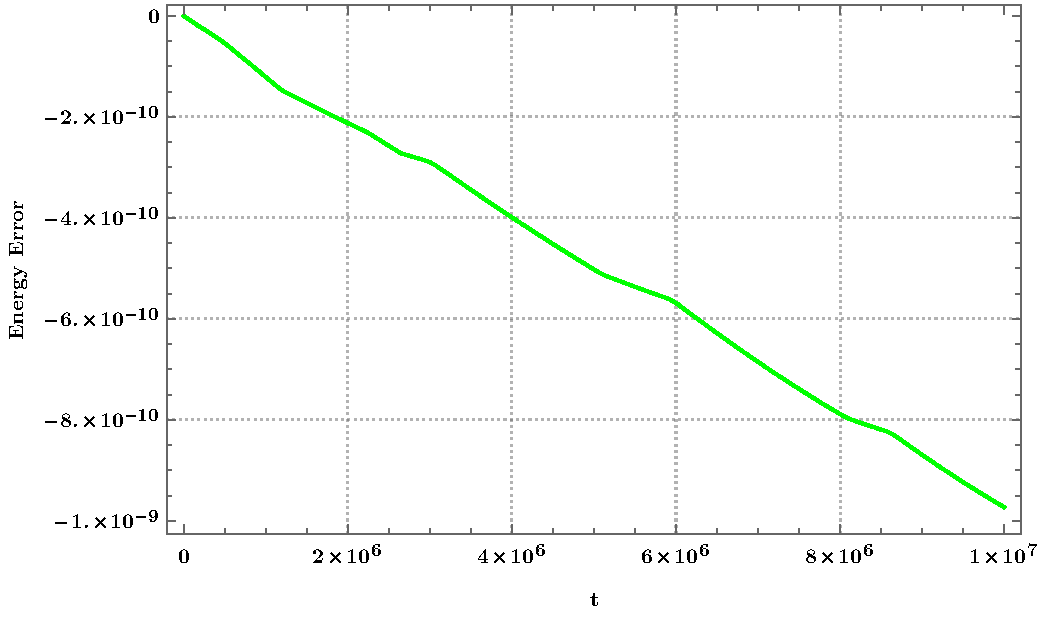
\includegraphics[width=.4\textwidth]{Fig1}}
&
\subfloat[OSS: New stopping criterion]
{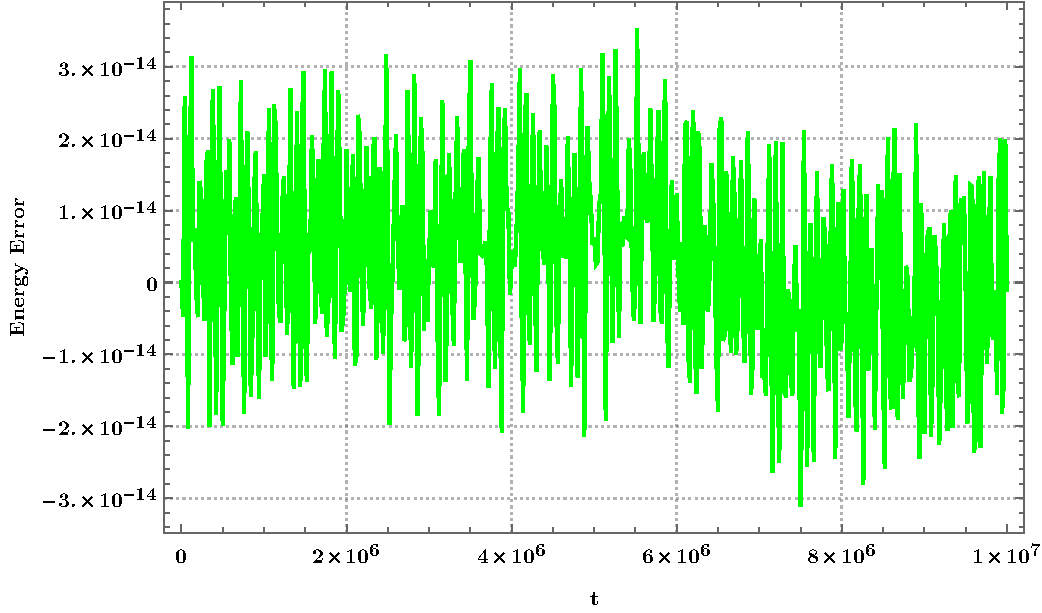
\includegraphics[width=.4\textwidth]{Fig2}}
\end{tabular}
\caption{\small Evolution of relative error in energy for the outer solar system problem (OSS) with the original unperturbed initial values in~\cite{Hairer2008} and doubled step-size ($h=1000/3$ days).  (a) Hairer's stopping criterion, (b) New stopping criterion}
\label{fig:OSSh2}
\end{figure}

Arazoari soluzioa emateko, geratze erizpidea berri bat proposatuko dugu. Honako notazioa finkatuko dugu,
\begin{equation*}
\Delta_j^{[k]}, \ \text{non} \ \Delta^{[k]} \in \mathbb{F}^{sd}  \ (1\leqslant j \leqslant sd).
\end{equation*}
 Iterazioak  $k=1,2,\ldots$ jarraitzea , $ \Delta^{[k]} =0$ bete arte edo honako baldintza bi iterazio jarraietan betetzen den artean,
\begin{equation}
\label{eq:not_stopping}
\forall j \in \{1,\ldots,s D\},  \quad
\min \left(\{|\Delta_j^{[1]}|,\cdots ,|\Delta_j^{[k-1]}|\} \ /\{0\} \right) \leqslant |\Delta_j^{[k]}|.
\end{equation}

Hairer-ek, eguzki-sistemaren kanpo planeten problemaren $h=1000/3$ eguneko urrats luzeerarekin egindako integrazioa errepikatu dugu baina oraingoan geratze erzipide berria aplikatuz. Energia errorearen eboluzioa (\ref{fig:OSSh2}Irudia) irudikatu dugu. 


\subsubsection*{Tolerantzi testa.}

Iterazio gehienetan, $j$ guztietarako $\Delta_{j}^{[k]}=0$ delako geratuko da. Dena den $j$ batetarako $\Delta_{j}^{[k]} \neq 0$ izanik iterazio geratzen bada, orduan puntu-finkoaren iterazioa onargarria den ala ez erabaki behar dugu. Iterazioa geratu daiteke biri


 orduan iterazio gehigarri bat emango dugu. Iterazio gehigarri bat emanez, esperimetanlki  puntu-finkoa lortzen den urratsen portzentaia nabarmen handitzen dela konprobatu dugu.


Puntu-finkoaren iterazioak amaitzerakoan, urratsa eman aurretik erabiltzaileak definitutako tolerantzia lortu den ala ez aztertuko dugu. Horretarako iterazioaren azken bi hurbilpenak konparatuko ditugu eta honako notazioa finkatuko dugu,

\begin{equation*}
Y_i=Y_i^{[k]}, \ \ \tilde{Y}_i=Y_i^{[k-1]}, \ \ i=1,\dots,s.
\end{equation*}  

Erabiltzaileak finkatutako tolerantzia erlatiboa eta tolerantzia absolutuaren parametroen arabera ($rto_i,atol_i, i=1,\dots,d$) , \emph{distantzia normalizatua} definituko dugu,
\begin{equation*}
\max_{i=1,\dots,d} \frac{\max_{j=1,\dots,s} |Y_j^i-\tilde{Y}_j^i|}
                        {\bigg(\big((\max_{j=1,\dots,s} |Y_j^i|+\max_{j=1,\dots,s} |\tilde{Y}_j^i|)/2 \big) \ rtol_i+ atol_i \bigg)}.
\end{equation*}

Distantzi normalizatua $>1$ bada orduan ez da lortu tolerantzia eta integrazio amaituko dugu.

Tolerantzia ez dugu erabiliko puntu-finkoko iterazio geratzeko, behin iterazioa geratu denean, emaitza onargarria den ala ez erabakitzeko baizik. Puntu-finkoko iterazioa konbergentzia lortu duelako edo konbergentzia arazoak izan direlako gera daiteke. Doitasun zehatzean, biribiltze errorearen eragina handia izan daiteke eta beraz, ez dugu tolerantzia estua erabiliko. Diskriminatu nahi dugu, aritmetika zehatzean konbergitu duen ala ez. Biribiltze errorea ez balitz konbergitu duen erabaki nahi dugu.

\subsection{Biribiltze errorea gutxitzeko teknikak (3.proposamena).}

Koma higikorreko aritmetika atalean (ikus \ref{sec:4.4}atala), baturan nahiz biderketan egindako biribiltze errore zehatza modu errazean kalkulatu daitekeela  ikusi genuen. Eragiketa hauen biribiltze erroreak, ondorengo konputazioetan erabiliko ditugu soluzioaren doitasuna hobetzeko.

Batura errekurtsiboetan, konputazioaren doitasuna hobetzeko teknikari \emph{batura konpensatua} esaten zaio eta zenbakizko integrazioetan erabili ohi da. Atal honetan, batetik IRK metodoetan batura konpensatuaren aplikazio estandarra hobetzeko proposamena azalduko dugu. Beste aldetik, IRK metodoaren gure  inplementazioan biribiltze errorearen beste jatorri nagusiak (biderketa eta batuketa bat) modu finagoan kalkulatzea proposatuko dugu.    

Goian aipatutako ideia,  beste ikuspegi batetik ere azaldu daiteke. Ikuspegi honen arabera, gure zenbakizko soluzioa, bi \emph{double} balioren bidez ($\tilde{y}_n,e_n$)  adierazten ari gara (ia doitasun laukoitza) eta beraz, interpretazio honen arabera, konputazio eragiketa batzuk ia doitasun laukoitzean egiten ariko ginateke. Zentzu honetan gure inplementazioan, hasierako balio zehatza $y_0=y(t_0)$, doitasun bikoitzeko bi zenbakiren bidez ($\tilde{y}_0, e_0$) hasieratuko dugu,
\begin{align*}
\tilde{y}_0 &=fl(y_0) ,\\
e_0 &=fl(y_0-\tilde{y}_0).
\end{align*}


\subsubsection*{Batura konpensatua (aportazioa).}

$y_{n+1} \in \mathbb{R}^{d},\quad y_{n+1}=\tilde y_{n}+\tilde \delta_n$ batura zehatza izanik eta $\tilde y_{n+1} \in \mathbb{F}^{d}, \quad \tilde y_{n+1}=\tilde y_{n} \oplus \tilde \delta_n$ koma-higikorreko hurbilpena izanik, batura konpensatuaren bidez lortutako errorearen estimazioa $e_{n+1}$ ,

\begin{algorithm}[H]
 \BlankLine
  $\tilde{y}_{0}=fl(y_{0}); \ e_0=fl(y_0-\tilde{y}_0)$\;
 \BlankLine
  \For{$n=1,2,\cdots \quad$}
  {
   \BlankLine
    $inc=\tilde {\delta}_n \oplus e_n$\;
    $\tilde {y}_{n+1}=\tilde{y}_n \oplus inc$\;
    $e_{n+1}=(\tilde{y}_n \ominus \tilde {y}_{n+1}) \oplus inc$\;
   \BlankLine
  }
 \caption{Batura konpensatua.}
\end{algorithm}

\paragraph*{}baturan egindako  biribiltze errore zehatza da,
\begin{equation}
y_{n+1}=\tilde {y}_{n+1}+e_{n+1}. 
\end{equation}

Horregatik, IRK metodoaren inplementazioan, inplizituki $Y_{n,i}$ atalak askatzeko ekuazioetan, $\tilde {y}_n$ ordez ($\tilde{y}_n \oplus \tilde{e}_{n}$) erabiltzea proposatzen dugu, 
\begin{equation}
\label{eq:eqbk}
L_{n,i}^{[k]}=hb_if(Y_{n,i}^{[k-1]}), \ \ \ Y_{n,i}^{[k]}=\tilde{y}_n \oplus \big(\tilde{e}_{n} \oplus \sum\limits_{j=1}^{s} \mu_{ij} L_{n,j}^{[k]}\big).
\end{equation}

Aldaketa honekin, lortutako zenbakizko soluzioaren doitasuna batura konpensatu estandarrarekin baino pixka bat hobea izango dela espero dugu. 

\subsubsection*{Biderketaren biribiltze errorea.}

Urratsa emateko unean, $L_{n,i}=hb_i \ f(Y_{n,i}), \ i=1,\dots,s$ biderketen biribiltze errorea kalkulatu eta $e_{n}$ gaiari gehituko diogu. Biderketaren biribiltze errorea jasotzeko konputagailuaren \emph{FMA} eragiketan oinarrituko gara eta (\ref{sec:4.4})ataleko (\ref{alg:FastSum}.algoritmoa) aplikatuko dugu. 

\begin{algorithm}[h]
$L_{n,i}^{[k]}=hb_i \ f(Y_{n,i}^{[k-1]})$\; 
$E_{n,i}=hb_i \ f(Y^{[k-1]}_{n,i}) - L^{[k]}_{n,i} \ \ , \ \ i=1,\dots,s$\;
$\beta_{n}={e}_{n} + \sum\limits_{j=1}^{s}E_{n,j}$\;
% \caption{Biderketaren biribiltze errorea eta batura konpensatua.}
\end{algorithm}

\subsubsection*{Baturaren biribiltze errorea.}

$\delta_n=\left(\sum\limits_{i=1}^{s}L_{n,i}^{[k]}\right)+\beta_{n}$ baturaren biribiltze errorea.


\begin{algorithm}[H]
  \SetAlgoLined\DontPrintSemicolon
  \SetKwFunction{algo}{algo}\SetKwFunction{BaturaKonpensatua}{BaturaKonpensatua}
  \SetKwProg{myalg}{Algorithm}{}{}
  \SetKwProg{myproc}{Function}{}{}
  \myproc{\BaturaKonpensatua {$y_n$,\ $\beta_n$,\ $L_n^{[k]}$}}{
     \BlankLine
     $s_0=y_n$\;
     $ee=\beta_n$\;
     \For{$i\leftarrow 1$ \KwTo ($s$)}
      {
        $s_1=s_0$\;
        $\delta= L_{n,i}^{[k]} +ee$\;
        $s_0=s_1+\delta$\;
        $ee=(s_1 - s_0)+ \delta$\;   
      }
     $y_{n+1}=s_0$\;
     $e_{n+1}=ee$\;    
    \KwRet ($y_{n+1}$,$e_{n+1}$) \;}
  \caption{BaturaKonpensatua}
\end{algorithm} 

\subsection{Biribiltze errorearen estimazioa (4.proposamena).}

Zenbakizko integrazioaren biribiltze errorearen estimazioa, bigarren zenbakizko integrazio baten soluzioaren diferentzia gisa kalkulatuko dugu. Bigarren integrazio honetan, $\tilde{\tilde{L}}_{n,i}$ terminoak mantisa txikiagoko zenbakira biribilduko ditugu,  doitasun gutxiagoko soluzioa lortzeko. 

$r\ge0$ zenbaki osoa, eta $x \in \mathbb{F}$ ($m$-biteko doitasuneko koma-higikorreko zenbakia) izanik, honako funtzioa definituko dugu,

\begin{algorithm}[H]
  \SetAlgoLined\DontPrintSemicolon
  \SetKwFunction{algo}{algo}\SetKwFunction{floatR}{floatR}
  \SetKwProg{myalg}{Algorithm}{}{}
  \SetKwProg{myproc}{Function}{}{}
  \myproc{\floatR {x,r}}{
    $res=(2^r x + x)- 2^r x$\;
    \KwRet res \;}
  \caption{floatR}
\end{algorithm} 

\paragraph*{}Funtzio honek itzultzen duen balioa, $(m-r)$-biteko doitasuneko koma-higikorreko zenbakia da. Beste modu batera esanda, $m$ biteko koma-higikorreko $x$ zenbakiaren azken $r$ bitak zeroan jartzen dituen funtzioa da.

Biribiltze errorearen estimazioa, zenbakizko soluzio nagusiaren $(y_n+e_{n})$ eta $r$ ($r<m$) balio txiki baterako (adibidez $r=3$) kalkulatutako bigarren zenbakizko soluzioaren $(\tilde{\tilde{y}}_n+\tilde{\tilde{e}}_{n})$ arteko diferentziaren norma bezala kalkulatuko dugu. 
\begin{equation}
estimazioa_n^i=\|(y_n^i+e_n^i)-(\tilde{\tilde{y}}_n^i+\tilde{\tilde{e}}_{n}^i)\|_2, \ \ i=1,\dots,d.
\end{equation}

Gure algoritmoan estimazioa zuzenean lortzeko, bi integrazioak sekuentzialki modu eraginkorrean kalkulatuko ditugu. Urrats bakoitzean, bi integrazioen $Y_i,\tilde{\tilde{Y}}_i$ ($i=1,\dots,s$) ataletako balioak, biribiltze errorea estimazio handiegia ez den artean,  antzekoak mantentzen dira. Beraz, bigarren integrazioan iterazio kopuru txikia beharko dugu, lehen integrazioaren bukaerako $Y_i^{[k]}$ ($i=1,\dots,s$) atalen balioak, bigarren integrazioaren $\tilde{\tilde{Y}}_i^{[0]}$ (i = 1, . . . , s) atalen hasieraketarako erabiltzen baditugu (ikus \ref{alg:errore-estimazioa}.algoritmoa).  

\begin{algorithm}[h!]
  \BlankLine
  \For{$n\leftarrow 0$ \KwTo ($endstep-1$)}
  {
    \BlankLine
    $Y_n^{[0]}=G(Y_{n-1},h)$\;
    \BlankLine
    $\text{Lehen Integrazioa}$\;
	\BlankLine
    $(y_{n+1},e_{n+1})\leftarrow BaturaKonpensatua(y_n,\beta_n,L_n^{[k]})$\;      
    \BlankLine
    \BlankLine
    \eIf{$(initwithfirst)$}
    {$\tilde{\tilde{Y}}_{n}^{[0]}=Y_{n}^{[k]}+(\tilde{\tilde{y}}_n-y_n)$\;}
    {$\tilde{\tilde{Y}}_{n}^{[0]}=G(\tilde{\tilde{Y}}_{n-1},h)$\;}
    \BlankLine
    $\text{Bigarren Integrazioa}$\;
	\BlankLine
    $(\tilde{\tilde{y}}_{n+1},\tilde{\tilde{e}}_{n+1})\leftarrow BaturaKonpensatua(\tilde{\tilde{y_n}},\tilde{\tilde{\beta}}_n,floatR(\tilde{\tilde{L}}_n^{[k]},r))$\;  
    \BlankLine
    \BlankLine
    $estimation_{n+1}=\|(y_{n+1}+e_{n+1})-(\tilde{\tilde{y}}_{n+1}-\tilde{\tilde{e}}_{n+1})\|_2$\;
    \BlankLine
   }
 \caption{RKG2: errore estimazioa}
 \label{alg:errore-estimazioa}
\end{algorithm}


\subsection{Algoritmoa.}

Formulazio berriari dagokion algoritmo orokorra laburtuko dugu \ref{alg:IRK-Berria}.algoritmoa.

\begin{algorithm}[h!]
 \BlankLine
  $\tilde{y}_0=fl(y_0)$\;
  $e_0=fl(y_0-\tilde{y}_0)$\;
  \For{$n\leftarrow 0$ \KwTo ($endstep-1$)}
  {
   \BlankLine
   $k=0$\;
   \text{Hasieratu}  $Y_{n,i}^{[0]} \ \ , \ \ i=1,\dots,s $\;
   \BlankLine
   \While{ (\text{not konbergentzia})}
   {
    \BlankLine 
    $k=k+1$\;
    $F_{n,i}^{[k]}=f(Y_{n,i}^{[k-1]}) $\;
    $L_{n,i}^{[k]}=hb_i \ F_{n,i}^{[k]} $\;
    $Y_{n.i}^{[k]}=\tilde{y}_{n} + \ \big(e_n+\sum\limits_{j=1}^{s} \mu_{ij} L_{n,j}^{[k]}\big)  $\;  
    $\text{konbergentzia} \leftarrow \text{GeratzeErizpidea}(Y^{[k]},Y^{[k-1]},\Delta_{min}) $\;
   }
   \BlankLine
   \If{($\exists j \ \text{non} \ \Delta_j^{[K]}\neq 0$)}
   {
   \If{$(NormalizeDistance(Y^{[k]},Y^{[k-1]})>1$}
   {$\text{fail convergence}$\;}
   }
   $E_{n,i} = h\,   b_i\,f_{n,i}^{[k]}-L_{n,i}^{[k]}$\;
   $\beta_{n}=e_{n}+\sum_{i=1}^{s} E_{n,i}$\;
   $(\tilde y_{n+1}, e_{n+1})\leftarrow \text{baturakonpensatua}(\tilde y_{n},\beta_{n},L_{n}^{[k]})$\;
   \BlankLine
 }
 \caption{IRK (puntu-finkoa).}
 \label{alg:IRK-Berria}
\end{algorithm}

\subsubsection*{Zenbakizko soluzioa.}  

Integrazio tartea $[t_0,t_{end}]$ eta urrats tamaina $h$ bada, emandako urrats kopurua $N=(t_{end}-t_0)/h$ izango da. Zenbakizko soluzioa fitxategi bitar batean idatziko da eta erabiltzaileak definitutako $m$ urratsero itzuliko da. 

$k$. integrazioan $N$ urrats eman baditugu eta $m$ finkatutako soluzioen frekuentzia bada, $t_i=t_0+i*(m \ h), \ i=1,\dots,N/m$ uneetarako zenbakizko soluzioa lortuko dugu. Bi integrazio mota exekutatu daitezke:

\begin{enumerate}
\item Integrazio arrunta.

Integrazioan itzultzen den fitxategiaren egitura honakoa da:
\begin{align*}
& (t_i,y_i,e_i) \ \text{non} \ \ y_i,e_i \in \mathbb{R}^d.\\
& y_i=(q_i,p_i) \ \text{eta} \ e_i=(eq_i,ep_i).
\end{align*}

\item Integrazioa errore estimazioarekin.

Errorearen estimazioa itzultzen duen integrazioaren emaitza honakoa da,
\begin{align*}
& (t_i,y_i,e_i,est_i) \ \text{non} \ \ y_i,e_i,est_i \in \mathbb{R}^d.\\
&  y_i=(q_i,p_i), \ e_i=(eq_i,ep_i) \ \text{eta} \ est_i=(estq_i,estp_i).
\end{align*}

\end{enumerate}

 Zenbakizko soluzioa doitasun bikoitzeko bi zenbakien batura gisa adieraziko dugu (aurretik azaldutakoaren erreferentzia),
\begin{equation*}
(y_i,e_i)=(q_i,p_i,eq_i,ep_i), \ \ y_i,e_i \in \mathbb{R}^d.
\end{equation*}
\begin{equation*}
(q_i^{[k]}+eq_i^{[k]},p_i^{[k]}+ep_i^{[k]})\approx(q(t_i)^{[k]},p(t_i)^{[k]}), \ \ \ i=1,\dots,N/m.
\end{equation*}


\clearpage

\section{Inplementazio estadarraren xehetasunak.}

\subsection*{Hamiltondar banagarriak.}

Era honetako ekuazio diferentzialak garrantzitsuak dira,
\begin{equation*}
\dot{p}=f(q), \ \ \dot{q}=g(p).
\end{equation*}

Esaterako, Hamiltondar banagarriak $H(q,p)=T(p)+U(q)$ eta bigarren ordeneko ekuazio diferentzialak $\ddot{q}=f(q)$ era honetako ekuazio diferentzialen kasu partikularrak dira.

Hurbilpena $(p_{n+1},q_{n+1}) \approx (p(t_{n+1}),q(t_{n+1}))$ era honetan kalkulatuko dugu,
\begin{align*}
p_{n+1}=p_n+ h \sum\limits_{i=1}^{s} b_i \ f(t_n+c_ih,Q_{n,i}),\\
q_{n+1}=q_n+ h \sum\limits_{i=1}^{s} b_i \ g(t_n+c_ih,P_{n,i}),
\end{align*}

non $(P_{n,i},Q_{n,i}), \ i=1,\dots,s$ honako ekuazio sistema definitutako atalak diren, 
\begin{align*}
P_{n,i} &=p_n+ h \sum\limits_{j=1}^{s} a_{ij} \ f(t_n+c_jh,Q_{n,j}), \\
Q_{n,i} &=q_n+ h \sum\limits_{j=1}^{s} a_{ij} \ g(t_n+c_jh,P_{n,j}).
\end{align*}

Era honetako problemetan,  funtsean \emph{IRK} algoritmo orokorra (alg.\ref{alg:IRK1}) aplikatuko dugu. Baina Hamiltondarraren egituraren abantaila aprobetxatuz, puntu-finkoaren iterazioaren konbergentzia hobetuko dugu,   

\begin{algorithm}[H]
  \For{ (k=1,2,\dots)}
  {
   $P_{n,i}^{[k]}=p_{n}+ h \ \sum\limits_{j=1}^{s} a_{ij} \ f(t_n+c_jh,Q_{n,j}^{[k-1]})$\; 
   $Q_{n,i}^{[k]}=q_{n}+ h \ \sum\limits_{j=1}^{s} a_{ij} \ g(t_n+c_jh,P_{n,j}^{[k]}), \ \ \ \ i=1,\dots,s $\; 
  }
 \caption{Puntu-finkoaren iterazioa (Gauss-Seidel).}
\end{algorithm}
 

\subsection*{Bigarren ordeneko EDA.}
 
 
Bigarren ordeneko ekuazio diferentzialen $\ddot{q}=f(q)$ (\emph{Runge-Kutta-Nyström}) azterketa egiteko, modu baliokide honetan idatziko dugu,
\begin{equation*}
\dot{p}=f(q), \ \ \dot{q}=p.
\end{equation*}

\paragraph*{}Hurbilpena $(p_{n+1},q_{n+1}) \approx (p(t_{n+1}),q(t_{n+1}))$ era honetan kalkulatuko dugu,
\begin{align*}
p_{n+1}=p_n+ h \sum\limits_{i=1}^{s} b_i \ f(t_n+c_ih,Q_{n,i}),\\
q_{n+1}=q_n+ h p_{n} + h^2 \sum\limits_{i=1}^{s} \beta_i \ f(t_n+c_ih,Q_{n,i}),
\end{align*}

non $Q_{n,i}, \ i=1,\dots,s$ honako ekuazio sistema definitutako atalak diren, 
\begin{align*}
Q_{n,i}=q_n+ h\gamma_i p_n+ h^2 \sum\limits_{j=1}^{s} \tilde{a}_{ij} \ f(t_n+c_jh,Q_{n,j}).
\end{align*}

\paragraph*{}{\textbf{IRK algoritmoa-III (bigarren ordeneko EDA)}.}


\begin{algorithm}[H]
 \BlankLine
  \For{$n\leftarrow 0$ \KwTo ($endstep-1$)}
  {
   \BlankLine
   Hasieratu  $Q_{n,i}^{[0]} \ \ , \ \ i=1,\dots,s $\;
    \BlankLine
   \While{ (konbergentzia lortu)}
   {
    \BlankLine 
    $F_{n,i}=f(t_n+c_ih,Q_{n,i}) \ \ , \ \  i=1,\dots,s$\;
    $Q_{n,i}=q_n+ h\gamma_i p_n+ h^2 \sum\limits_{j=1}^{s} \tilde{a}_{ij} \ f(t_n+c_jh,Q_{n,j}) \ \ , \ \  i=1,\dots,s$\;  
   }
   \BlankLine
    $\delta p_n=h \ \sum\limits_{i=1}^{s} b_i F_{n,i}$\;
    $\delta q_n=h^2 \sum\limits_{i=1}^{s} \beta_i F_{n,i}$\;    
    $p_{n+1}=p_{n}+ \delta p_n $\;
    $q_{n+1}=q_{n}+ h\gamma_i p_n+\delta q_n $\;
   \BlankLine
 }
 \caption{IRK algoritmoa-III (bigarren ordeneko EDA)}\label{alg:IRK2}
\end{algorithm}

\paragraph*{}Bigarren ordeneko ekuazio diferentzialak ditugunean, puntu-finkoko iterazioa,

\begin{algorithm}[H]
  \For{ (k=1,2,\dots)}
  {
   $Q_{n,i}^{[k]}=q_{n}+h \gamma_i p_{n}+ h^2 \ \sum\limits_{j=1}^{s} \tilde{a}_{ij} f(t_n+c_jh,Q_{n,j}^{[k-1]}) $\;  
  }
 \caption{Puntu-finkoko iterazioa (bigarren ordeneko EDA)}
\end{algorithm} 


\section{Esperimentuak.}

\subsection{Sarrera.}

Lau problemetarako esperimentuetan, integrazio parametroak bateratu ditugu. 

\begin{enumerate}

\item $s=6$ ataletako Gauss IRK metodoa aplikatu dugu.

\item Epe luzeko integrazioak aztertu ditugu.

\item Urratsa, trunkatze errorea biribiltze errorea baino txikiagoa izan dadin aukeratu dugu. 

\item Integrazio mota bakoitza $P=1.000$ perturbatutako hasierako balio ezberdinekin integratu dugu. Perturbazioen kalkulurako $k=2^{-20}$ balioa finkatu dugu, hau da, $\mathcal{O}(10^{-16})$   mailako perturbazioak aplikatu ditugu problema guztietarako.  

\item Kokapen errorearen estimazioaren kalkuluan, integrazio nagusian $rdigits1=0$ eta bigarren integrazioan $rdigits2=3$ balioak erabili ditugu.

\end{enumerate}

Lau probema ezberdinetarako egin ditugu zenbakizko esperimentuak eta bakoitzean zehazki erabilitako integrazio tartea eta urratsa tamainak hauek izan dira:

\begin{enumerate}
\item Pendulu bikoitza ez-kaotikoa (NCDP).
\begin{align*}
& t_0=0, \ \ t_{end}=2^{12}, h=2.^{-7}, \\
& m=2^{10}, L=512.
\end{align*} 

\item Pendulu bikoitza kaotikoa (CDP).
\begin{align*}
& t_0=0, \ \ t_{end}=2^{8}, h=2.^{-7}, \\
& m=2^6, L=512.
\end{align*} 

\item Outer solar system (6-Body).
\begin{align*}
& t_0=0, \ \ t_{end}=10^{7}, h=500/3, \\
& m=120, L=500.
\end{align*} 

\item Solar system (10-Body).
\begin{align*}
& t_0=0, \ \ t_{end}=10^{6}, h=2, \\
& m=2000, L=250.
\end{align*} 

\end{enumerate}

\subsection{Energia errore jatorriak.}

Gure doitasun bikoitzeko inplementazioaren zenbakizko soluzioaren $\tilde{y}_n+e_n \approxeq y(t_n) \ (n=1,2,\cdots)$ errorea, jatorri ezberdineko errore mota ezberdinen konbinazioa da:

\begin{enumerate}
\item Trunkatze errorea. Hasierako baliodun problemaren soluzio zehatza $y(t_n)$, ($n=1,2,3,\cdots$), (\ref{eq:irk}) metodoa aplikatuz  ($b_i,\mu_{ij}$ koefiziente zehatzekin) lortutako zenbakizko soluzioa $y_n$ ordezkatzerakoan eragindako errorea. 
\item Iterazio errorea. Praktikan, puntu-finkoko iterazioa (\ref{alg:pf}) $K$ kopuru finitua aplikatzen da, eta $L_{n.i}, Y_{n,i} \ (i=1,\cdot,s)$ soluzioa, $L_{n.i}^{[K]}, Y_{n,i}^{[K]}$ hurbilpenarekin ordezkatzen da. Hurbilpen honen arabera dagokion zenbakizko soluzioa kalkulatzen da,
\begin{equation*}
y_{n+1}=y_{n}+\sum_{i=1}^{s} L_{n,i}^{[K]}.
\end{equation*}   
\item Funtzioa zehatza $f:\mathbb{R}^D \rightarrow \mathbb{R}^D$, bere doitasun bikoitzeko bertsioaz $\tilde{f}:\mathbb{F}^D \rightarrow \mathbb{F}^D$ ordezkatzerakoan eragindako bi mailetako errorea. Batetik, $K$ iterazio finituetan puntu-finkora iristeagatik eragindako ekidin ezineko iterazio errorea. Bestetik, $\tilde{f}$ konputazioan gertatutako biribiltze erroreak. 
\item IRK metodoaren koefiziente zehatzak $b_i,\mu_{ij} \in \mathbb{R}$, dagozkien doitasun bikoitzeko koefiziente $\tilde{b}_i,\tilde{\mu}_{ij} \in \mathbb{F}$ erabiltzeagatik eragindako errorea.
\item Algoritmoaren inplementazioaren eragiketa aritmetikoak, doitasun bikoitzean kalkulatzeagatik eragindako errorea.  
\end{enumerate} 

Errore jatorri hauek energian duten eragina simulatzeko, honako algoritmoak inplementatu ditugu:

\begin{enumerate}

\item Inplementazio zehatza.

Konputazio guztia (ekuazio diferentzialaren funtzioaren ebaluazioa barne) doitasun laukoitzeko ($128$-bit) koma higikorreko aritmetikan  egindako integrazioa. Zenbakizko integrazio hau, trunkatze errorea estimatzeko eta errore globala kalkulatzeko erreferentzi gisa (soluzio zehatza) kontsideratuko dugu. 

\item Inplementazio superideala.

Zenbakizko integrazio hau iterazio errorea estimatzeko erabiliko dugu. Konputazio guztia doitasun laukoitzean egindako integrazioa baina geratze erizpidea, doitasun bikoitzean neurtuko dugu,
\begin{equation*}
\Delta^{[k]}=|\text{double}(Y^{[k]})-\text{double}(Y^{[k-1]})|.
\end{equation*}

\item Inplementazio ideala.

Ekuazio diferentzialaren eskuin aldeko funtzioaren ebaluazioa izan ezik, beste eragiketa guztiak doitasun laukoitzean egiten dituen inplementazioa da. Ekuazio diferentziala doitasun bikoitzean kalkulatzeak, eragiten duen errorea neurtzeko erabiliko dugu eta integrazio hau hobetu ezin daitekeen integrazioa kontsideratuko dugu.  

\item Inplementazio sasi-ideala.

Doitasun bikoitzeko koefizienteak ($\tilde{\mu}_ij,\tilde{b}_i \in \mathbb{F}$) erabiltzeak eragiten duen errorea neurtzeko integrazioa da. Konputazio guztia doitasun laukoitzean kalkulatzen da baina doitasun bikoitzeko koefizienteen balioak erabiliz (doitasun bikoitzeko koefiziente koadrifikatuak esaten diogu). 

\end{enumerate}

We next plot (Fig. \ref{fig:SourceError}), for each of the three considered initial value problems, the evolutions of the energy errors corresponding to the items A--D in previous list. We confirm that for the time-step $h$ considered, truncation error is below round-error. The use of double precision coefficients ($\tilde{b}_i, \tilde{\mu}_{ij}$) is do not effect in the propagation of round-off. The iteration error is very similar to the round-off error and it could be cause an energy drift. 

\begin{figure}[h]
\centering
\begin{tabular}{c c}
\subfloat[NCDP ($h=2^{-7}$)]
{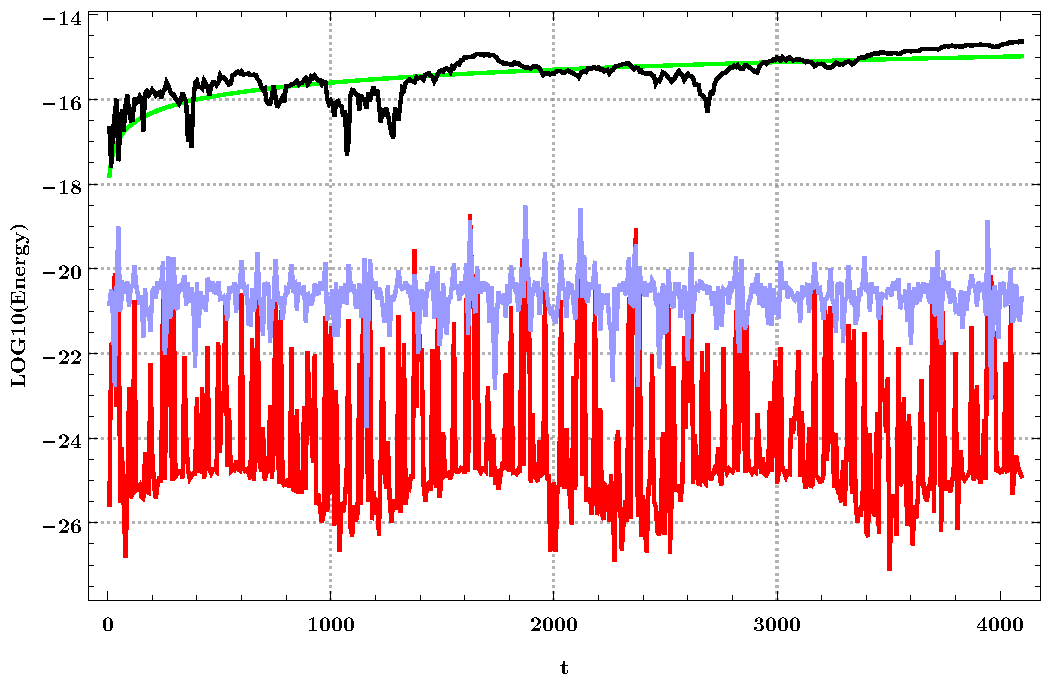
\includegraphics[width=.400\textwidth]{NCDP1A}}
&
\subfloat[NCDP ($h=2^{-7}/2$)]
{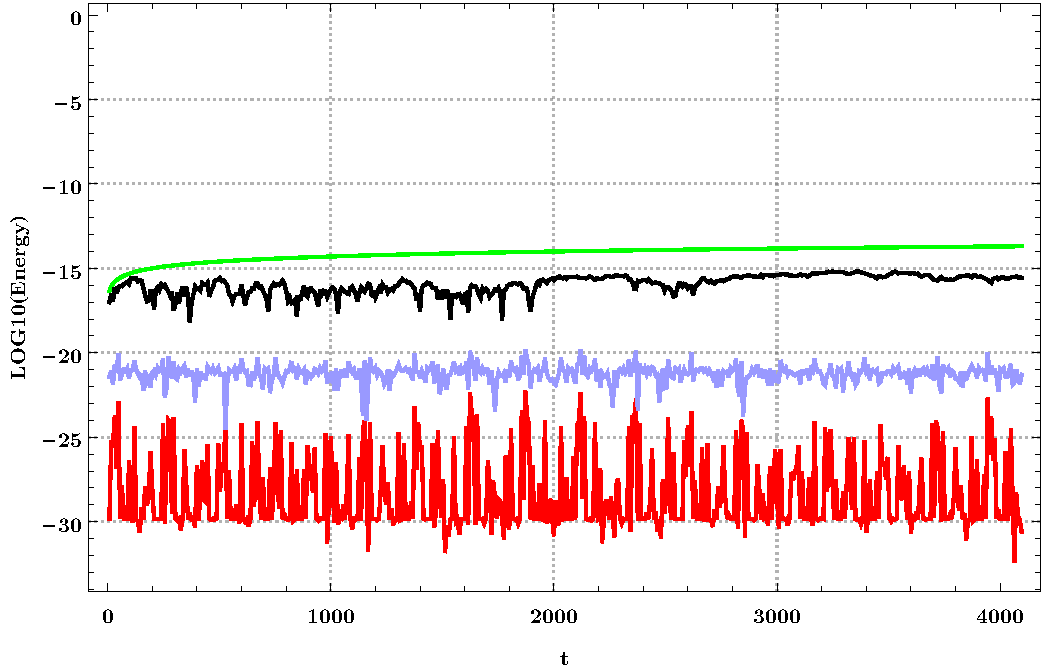
\includegraphics[width=.400\textwidth]{NCDP1B}} \\
% Zerbitzaria/1-Artikulua-Esperimentuak-4B/12-Esperimentua-V11/Experiments
\subfloat[CDP ($h=2^{-7}$)]
{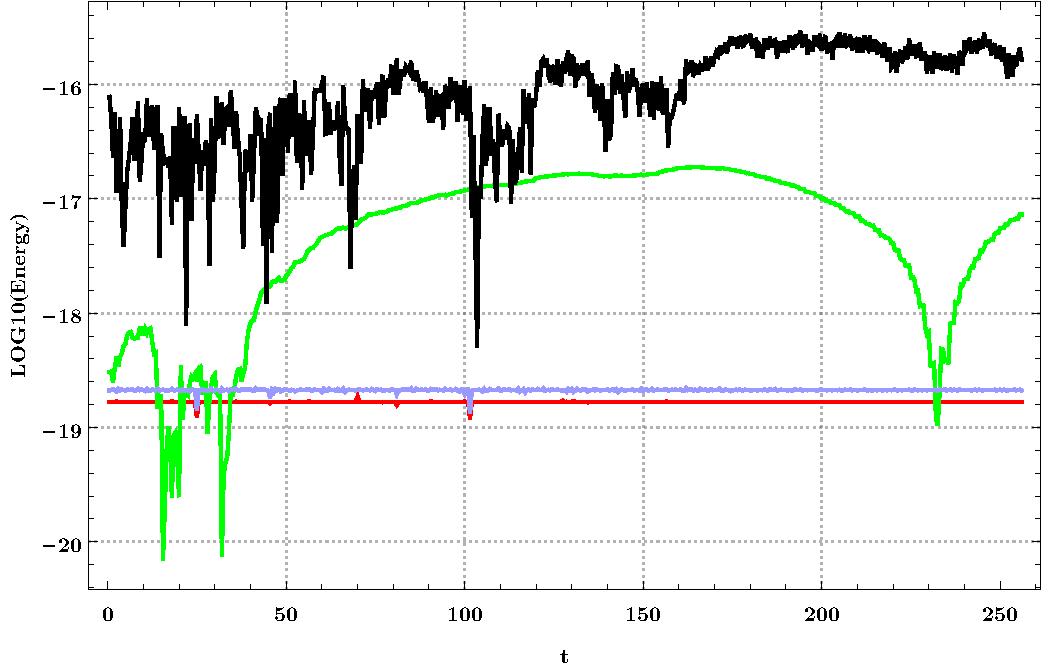
\includegraphics[width=.400\textwidth]{CDP1A}}
&
\subfloat[CDP ($h=2^{-7}/2$)]
{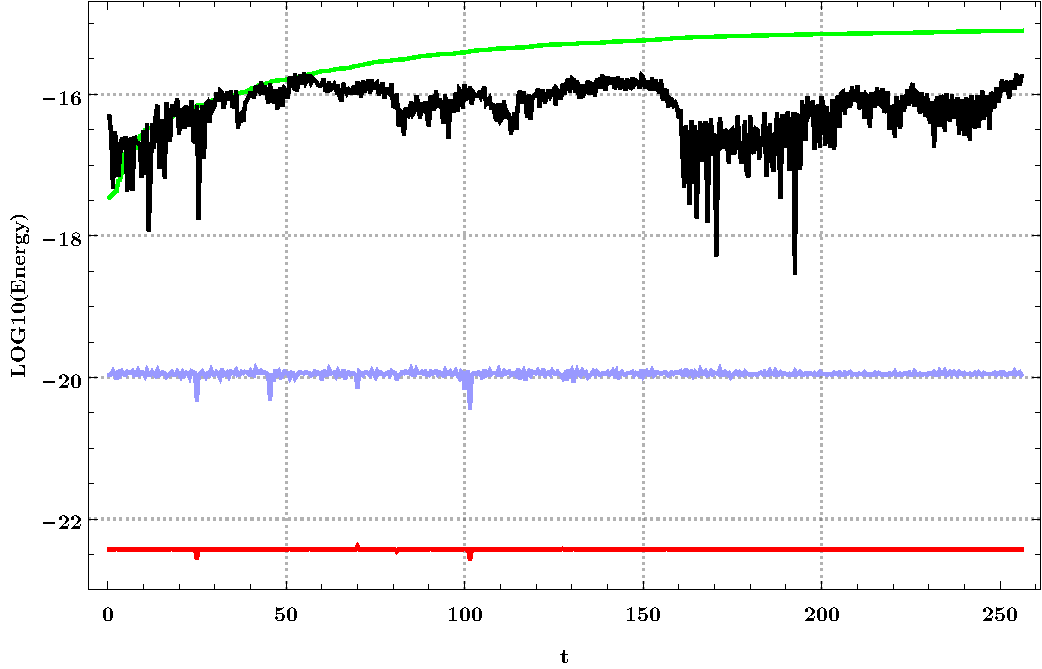
\includegraphics[width=.400\textwidth]{CDP1B}} \\
% Zerbitzaria/1-Artikulua-Esperimentuak-4B/13-Esperimentua-V12/Experiments
\subfloat[6-body ($h=500/3$)]
{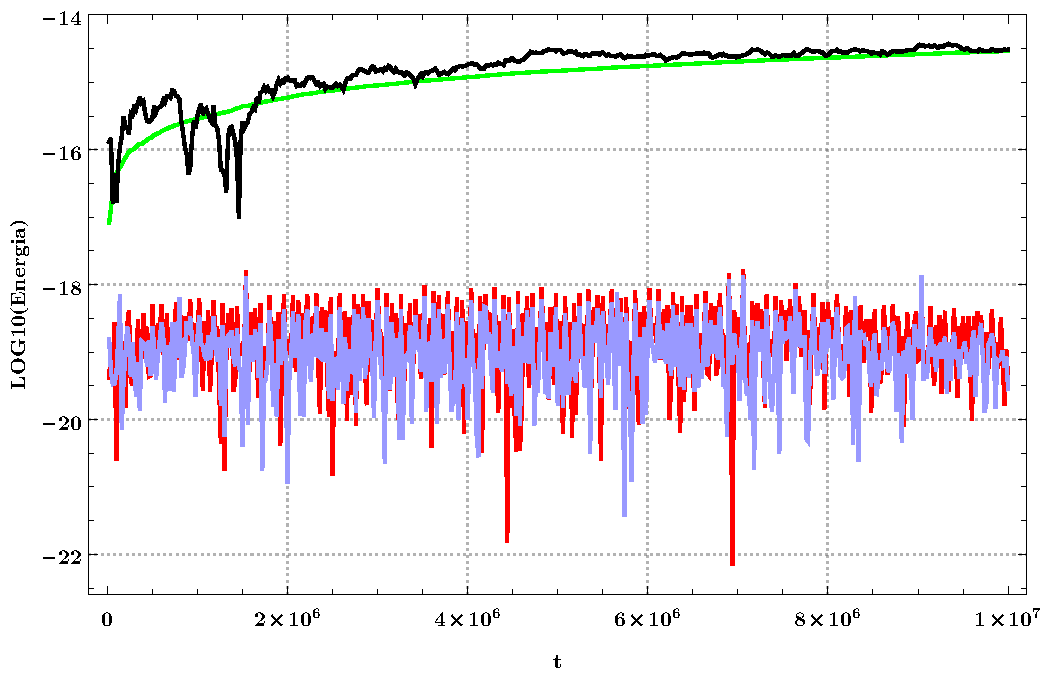
\includegraphics[width=.400\textwidth]{NBODY1A}}
&
\subfloat[6-body ($h=500/6$)]
{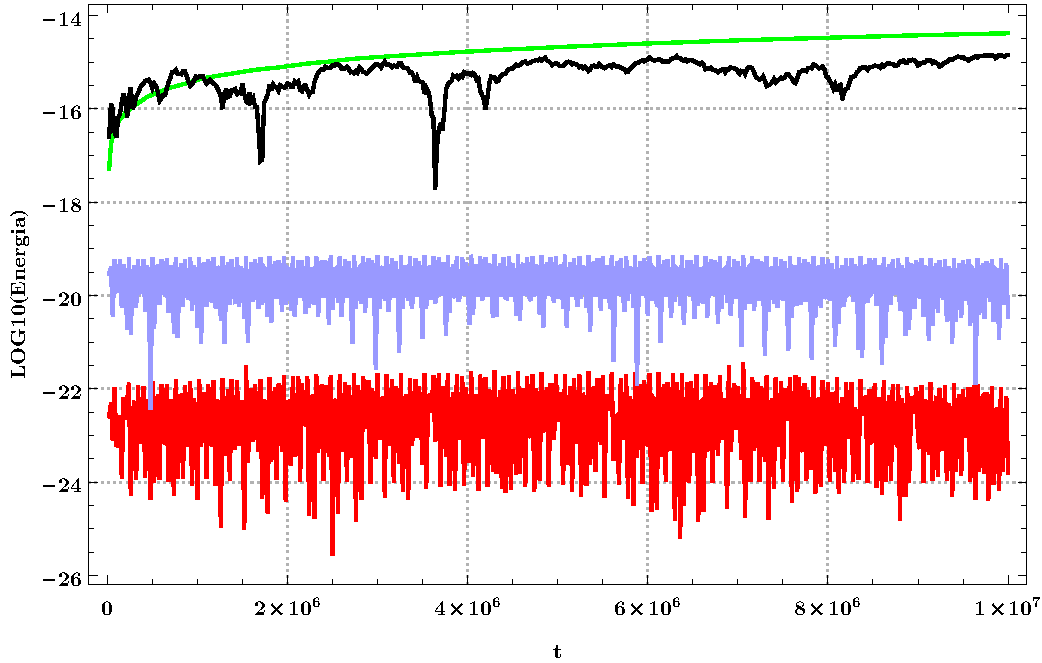
\includegraphics[width=.400\textwidth]{NBODY1B}} \\
%Zerbitzaria/1-Artikulua-Esperimentuak-4B/11-Esperimentua-V102/Esperiments
\subfloat[10-body ($h=2$)]
{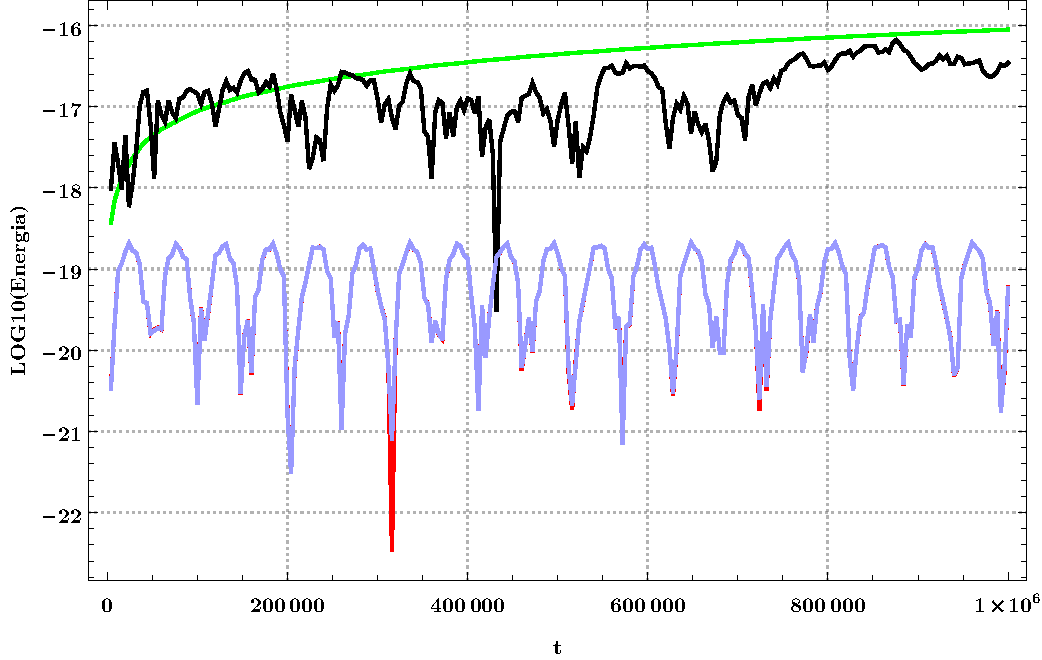
\includegraphics[width=.400\textwidth]{10NBODY1A}}
&
\subfloat[10-body ($h=1$)]
{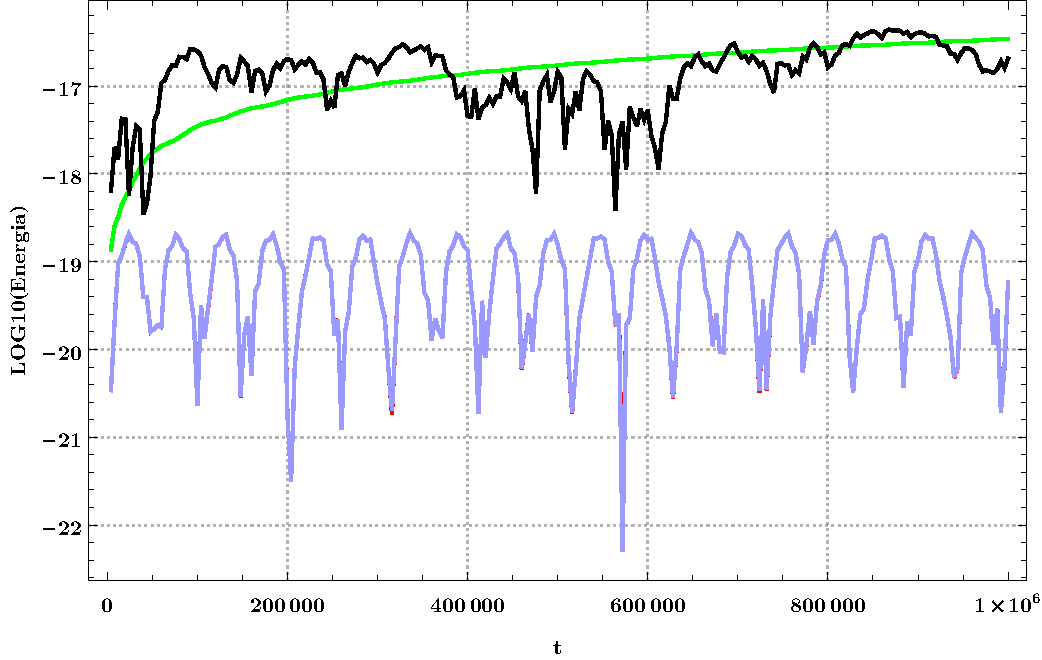
\includegraphics[width=.400\textwidth]{10NBODY1B}}
%Zerbitzaria/1-Artikulua-Esperimentuak-4B/11-Esperimentua-V102/Esperiments
\end{tabular}
\caption{\small We plot the evolution of energy relative error in logarithmic scale of the next algorithms implementations: A-algorithm  as estimation of truncation error (red), B-algorithm  as estimation of iteration error (green), C-algorithm  as estimation of the effect of the computation of double precision $\tilde{f}$ function (black) and D-algorithm  as estimation of the effect of using double precision $\tilde{b}_i, \tilde{\mu}_{ij} \in \mathbb{F}$ coefficients (blue). We show an figure for each initial value problem: Double Pendulum Non-Chaotic case (a), Double Pendulum Chaotic case (b) and outer solar system case (e).}    
\label{fig:SourceError}
\end{figure}

\subsection{Errore azterketa estadistikoa.}

Errorearen konparaketa fidagarriagoa egiteko helburuarekin,  azterketa estadistikoa egin dugu. Ausaz perturbatutako $P=1000$ hasierako balio ezberdinetarako integrazioak exekutatu ditugu eta emaitza hauen guztien batezbestekoan oinarritu gara, biribiltze errorearen azterketa egokia egiteko.    

\paragraph*{Ausazko perturbazioak.}
Perturbaziorik gabeko hasierako balioa $(u0,e0)$ eta $\mathcal{O}(10^{-6})$ ordeneko $k$ perturbazio tamaina finkatuta, era honetan kalkulatuko dugu $(u1D,e1)$ perturbatutako hasierako balioa,
\begin{lstlisting} [language=Mathematica]
k = 2^(-20);
u1 = u0 + u0*(k*RandomReal[{-1,1}]);
u1D = N[u1];
u1DD = SetPrecision[u1D, prec];
e1 = N[u1 - u1DD];
\end{lstlisting}

\paragraph*{}Puntu-finko interazio bidezko $6$-ataletako Gauss kolokazio metodoaren hiru inplementazio konparatu ditugu:

\begin{enumerate}
\item Inplementazio ideala. Ekuazio diferentzialaren eskuin aldeko funtzioaren ebaluazioa izan ezik, beste eragiketa guztiak doitasun laukoitzean egiten dituen inplementazioa da.

\item Doitasun bikoitzeko gure inplementazioa berria (DP).

\item Hairer-en inplementazioa ~\cite{Hairer2008}, jatorrizko bere IRK metodoaren Fortran kodea exekutatu dugu (\href{http://www.unige.ch/~hairer/preprints.html}{Hairer's preprints page}).     

\end{enumerate}

\begin{table}
\caption[Fixed-point percentage of steps and mean iterations.] 
{\small{Percentage of steps that reach a computational fixed-point and the number of fixed-point iterations per step for the computations of non-chaotic double pendulum (NCDP), chaotic double pendulum (CDP), and the outer solar system (OSS) problems. In columns, we compare three different implementations: FPIEA (ideal), DP (double precision) and Hairer's Fortran code.}}
\label{tab:fp}       % Give a unique label
\centering
%\resizebox{\textwidth}{!}
{%
\begin{tabular}{ l c c c c c c } 
 \hline
                 &  \multicolumn{2}{c}{FPIEA}  & \multicolumn{2}{c}{DP} & \multicolumn{2}{c}{Hairer} \\
 \hline
 NCDP            & $98.7\%$    & $9.5$   & $98.8\%$     & $8.6$   &  $98.5\%$ & $8.6$  \\ 
 CDP             & $98.9\%$    & $9.5$   & $98.9\%$     & $8.6$   &  $98.4\%$ & $8.6$  \\ 
 OSS             & $97.4\%$    & $15.2$  & $97.4\%$     & $14.2$  &  $87.5\%$ & $14.1$ \\ 
   \hline
 \end{tabular}}
 \end{table}


\subsubsection*{Distribution of energy jumps.}

Integratzailearen inplementazio egoki batean, biribiltze erroreak eragindako energiaren errore lokala $H(y_n)-H(y_{n-1}$), ausazkoa izatea espero da. Zenbakizko soluzioa $m$ urratsero jasotzen dugula jakinik, energi diferentzia $H(y_{km})-H(y_{km-m})$ ausazkoa izango da, $\mu$ batazbestekoa ($\mu=0$ ideala) eta $\sigma$ duen distribuzio Gausiarrarekin. Beraz, metatutako energia diferentzia
\begin{equation*}
H(y_{km})-H(y_0),
\end{equation*} 
$t_{mk}=t_0+kmh$ uneetarako, $k^{1/2} \sigma=(t_{mk}/(mh))^{1/2} \sigma$ desbiazio estandarra duen ausazko ibilbide Gausiar bat (\emph{random walk}) jarraituko du. Brouwer-ek Kepler problemarentzat zenbakizko integrazioaren birbiltze errorearen azterketa egin zuen ~\cite{Brouwer1937} eta horregatik, aurretik aipatutakoa Brouwer legea bezala ezaguna da konputazio zientzian ~\cite{Grazier2005}.

Integrazio tartea $[t_0, t_{end}]$ bada eta $P$ perturbatutako hasierako balio kopurua bada, $L \ P$ energia diferentzia balioak ditugu,
\begin{equation*}
\frac{H(y_{km})-H(y_{km-m})}{H(y_0)},
\end{equation*} 
non $L=(t_{end}-t_0)/(mh)$ den. (\ref{fig:hist}) irudian, $L \ P$ balioen histogramak eta $N(\mu,\sigma)$ distribuzio normalak irudikatu ditugu (non $\mu$ eta $\sigma$, balioei dagokien batazbestekoa eta desbiazio tipikoak diren). Gure helburua , gure DP inplementazioari dagozkion histogramak distribuzio Gausiarra ondo egokitzen zaion ikustea da.    

\begin{figure}[h!]
\centering
\begin{tabular}{c c}
\subfloat[\small {NCDP : FPIEA.}]
{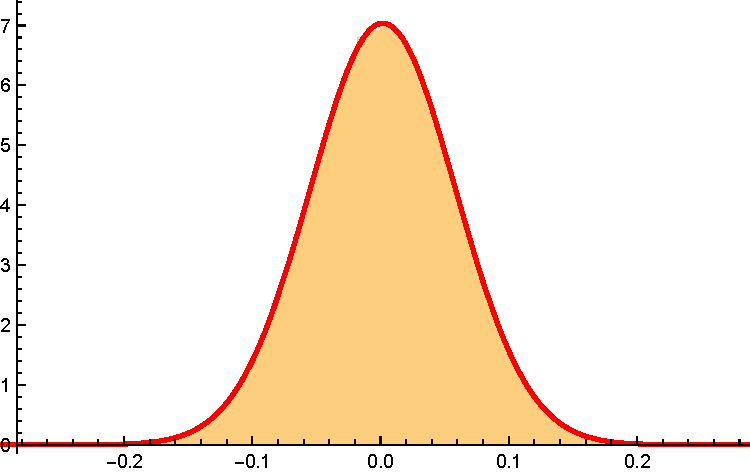
\includegraphics[width=.4 \textwidth]{NCDP2A}}
&
\subfloat[\small {NCDP : DP.}]
{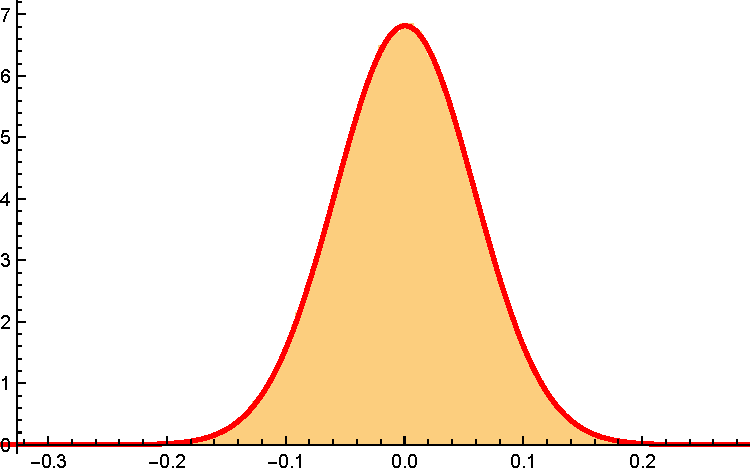
\includegraphics[width=.4\textwidth]{NCDP2B}}
\\
$(\mu=1.8\mathbf{e}{-18}$, \ $\sigma=1.5\mathbf{e}{-17}$) & ($\mu=5.3\mathbf{e}{-19}$, \ $\sigma=1.5\mathbf{e}{-17}$)\\
% Zerbitzaria/1-Artikulua-Esperimentuak-4B/13-Esperimentua-V122/Experiments/NCDP-ZAHAR
%
\subfloat[CDP : FPIEA.]
{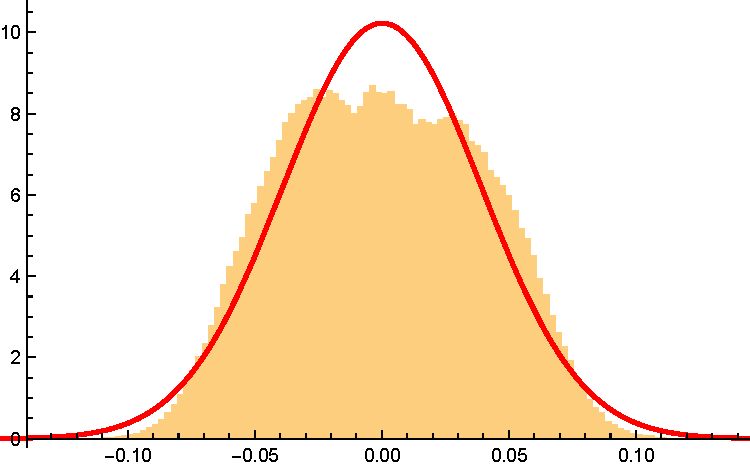
\includegraphics[width=.4\textwidth]{CDP2A}}
&
\subfloat[CDP : DP.]
{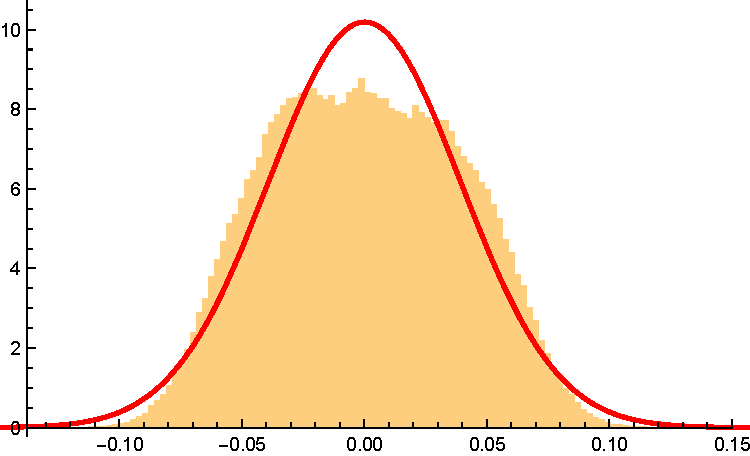
\includegraphics[width=.4\textwidth]{CDP2B}}
%
\\
$(\mu=1.6\mathbf{e}{-19}$, \ $\sigma=2.6\mathbf{e}{-17}$) & ($\mu=1.4\mathbf{e}{-19}$, \ $\sigma=2.6\mathbf{e}{-17}$)\\
% Zerbitzaria/1-Artikulua-Esperimentuak-4B/13-Esperimentua-V12/Experiments
%
\subfloat[6-Body : FPIEA.]
{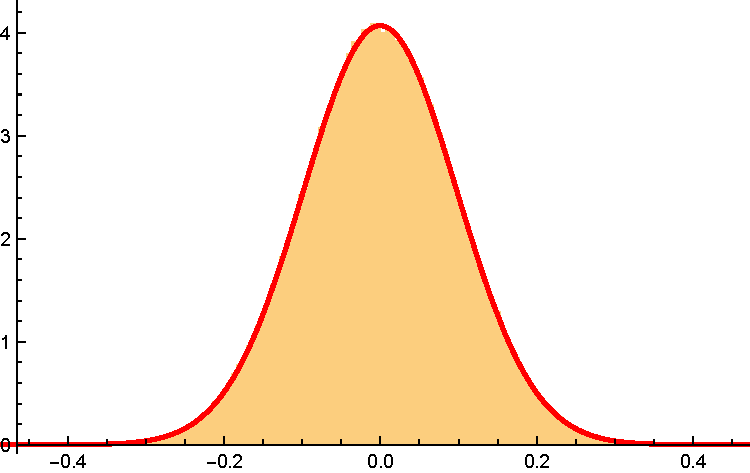
\includegraphics[width=.4\textwidth]{NBODY2A}}
&
\subfloat[6-Body : DP.]
{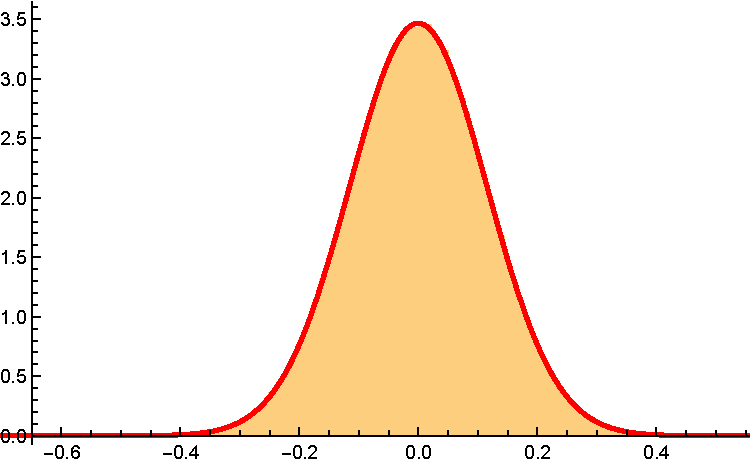
\includegraphics[width=.4\textwidth]{NBODY2B}}
\\
$(\mu={-3.2}\mathbf{e}{-19}$, \ $\sigma=3.3\mathbf{e}{-18}$) & ($\mu=-1.9\mathbf{e}{-19}$, \ $\sigma=3.5\mathbf{e}{-18}$)\\
% Zerbitzaria/1-Artikulua-Esperimentuak-4B/13-Esperimentua-V122/Experiments/6-Body (approx=1)
%
\subfloat[10-Body : FPIEA.]
{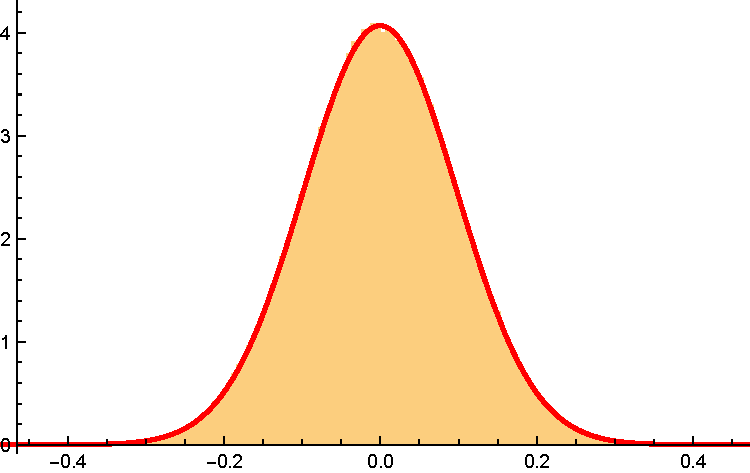
\includegraphics[width=.4\textwidth]{NBODY2A}}
&
\subfloat[10-Body : DP.]
{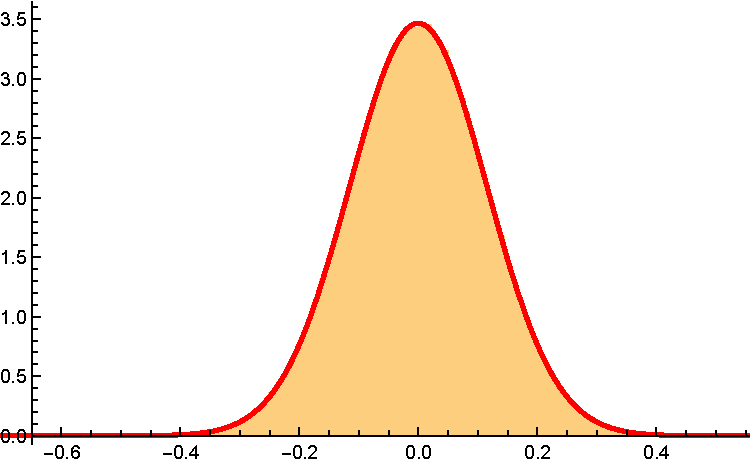
\includegraphics[width=.4\textwidth]{NBODY2B}}
\\
$(\mu={-3.2}\mathbf{e}{-19}$, \ $\sigma=3.3\mathbf{e}{-18}$) & ($\mu=-1.9\mathbf{e}{-19}$, \ $\sigma=3.5\mathbf{e}{-18}$)
% Zerbitzaria/1-Artikulua-Esperimentuak-4B/13-Esperimentua-V122/Experiments/6-Body (approx=1)
%
\end{tabular}
\caption{ \small Histograms of $K P$ samples of energy jumps against the normal distribution $N(\mu, \delta)$. The horizontal axis is multiplied by $10^{15}$ and vertical axis ???. for the FPIEA and  DP implementations for the three considered problems (NCDP, CDP, and OSS).}
\label{fig:hist}
\end{figure}

\subsubsection*{Evolution of mean and standard deviation of errors}


(\ref{fig:Htt}) irudian, energiaren errorearen batazbestekoa eta desbiazio tipikoa irudikatu ditugu.
\begin{align*}
&\Delta E_i^{[k]} =\frac{(E^{[k]}_i-E^{[k]}_0)}{E^{[k]}_0}, \ \ \ i=1,\dots,N/m \ \text{eta} \ k=1,\dots,P.\\
&\bar{\Delta E_i} =\frac{1}{P} \sum_{k=1}^{P} \Delta E_i^{[k]}, \ \  \sigma_i =\sqrt{\frac{1}{P} \sum_{k=1}^{P} (\Delta E_i^{[k]}-\bar{\Delta E_i})^2}.
\end{align*} 

eta kokapen erroreak: doitasun laukoitzean lortutako soluzioa, soluzio zehatza kontsideratuko dugu,           
\begin{equation*}
yexact^{[k]}_i=\hat{y}^{[k]}_i=(\hat{q}^{[k]}_i+\hat{eq}^{[k]}_i,\hat{p}^{[k]}_i+\hat{ep}^{[k]}_i),\ \ i=1,\dots,N/m .
\end{equation*}

eta $k.$ soluzioari ${y}^{[k]}_i=({q}^{[k]}_i+{eq}^{[k]}_i,{p}^{[k]}_i+{ep}^{[k]}_i)$ dagokion kokapen errorea,          
\begin{align*}
&Ge^{[k]}_i =\|(\hat{q}^{[k]}_i+\hat{eq}^{[k]}_i)-(q^{[k]}_i+eq^{[k]}_i)\|_2.
\end{align*}  

\begin{figure}[h!]
\centering
\begin{tabular}{c c}
\subfloat[NCDP: energy error]
{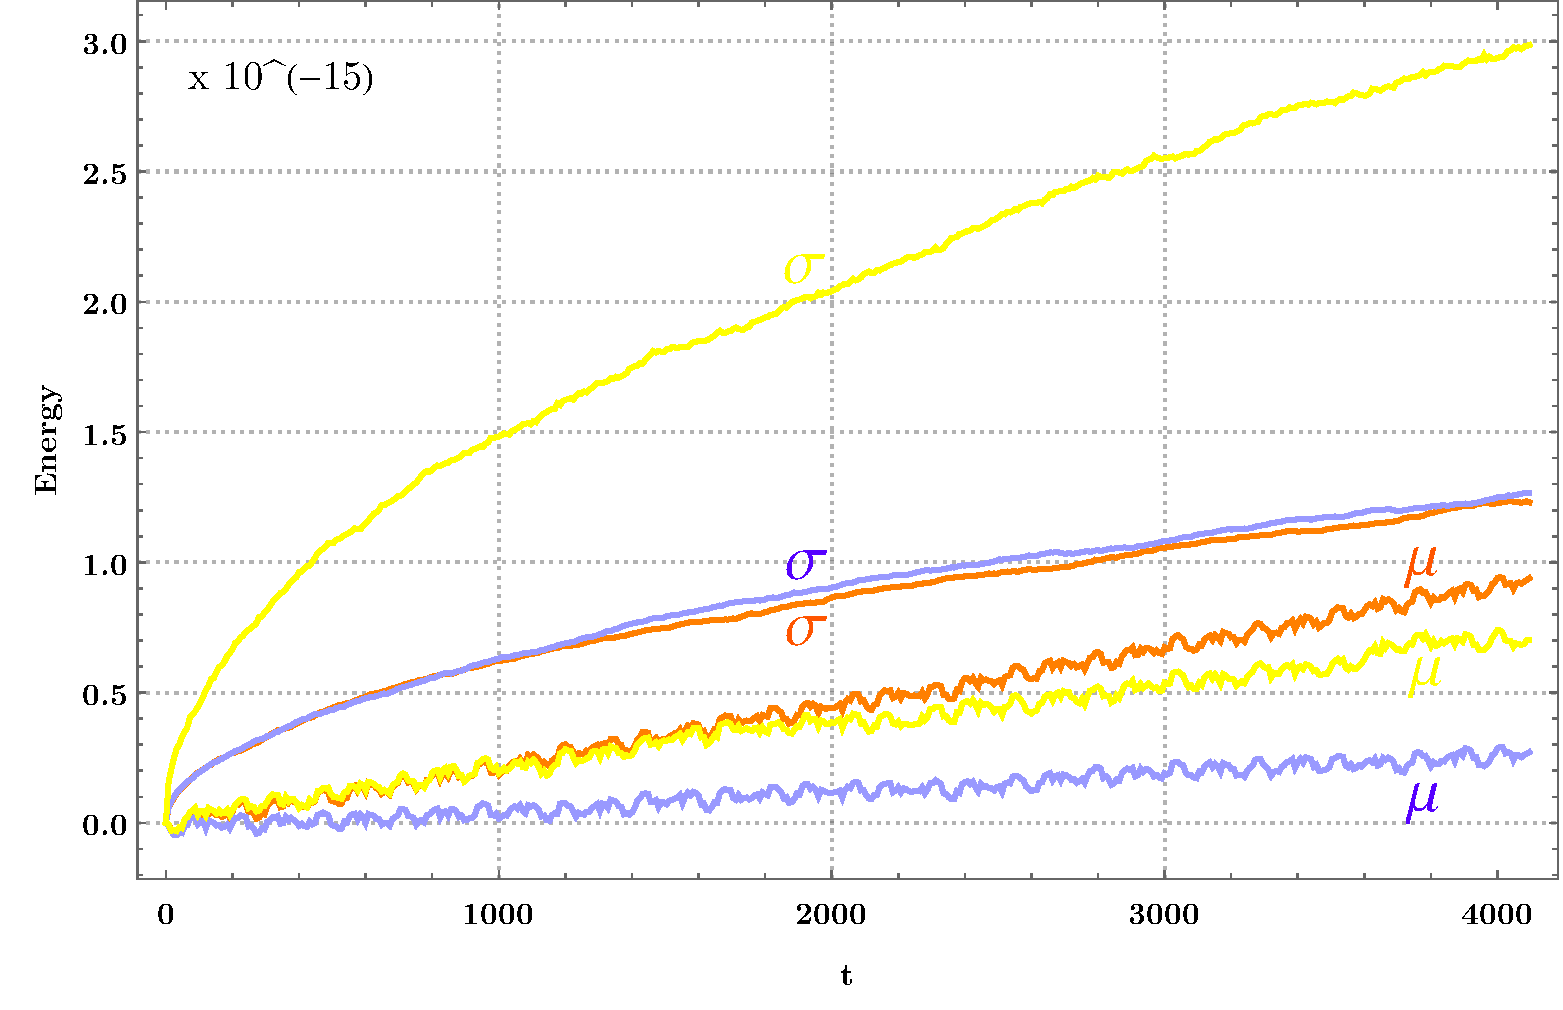
\includegraphics[width=.4\textwidth]{NCDP3A}}
&
\subfloat[NCDP: mean global error.]
{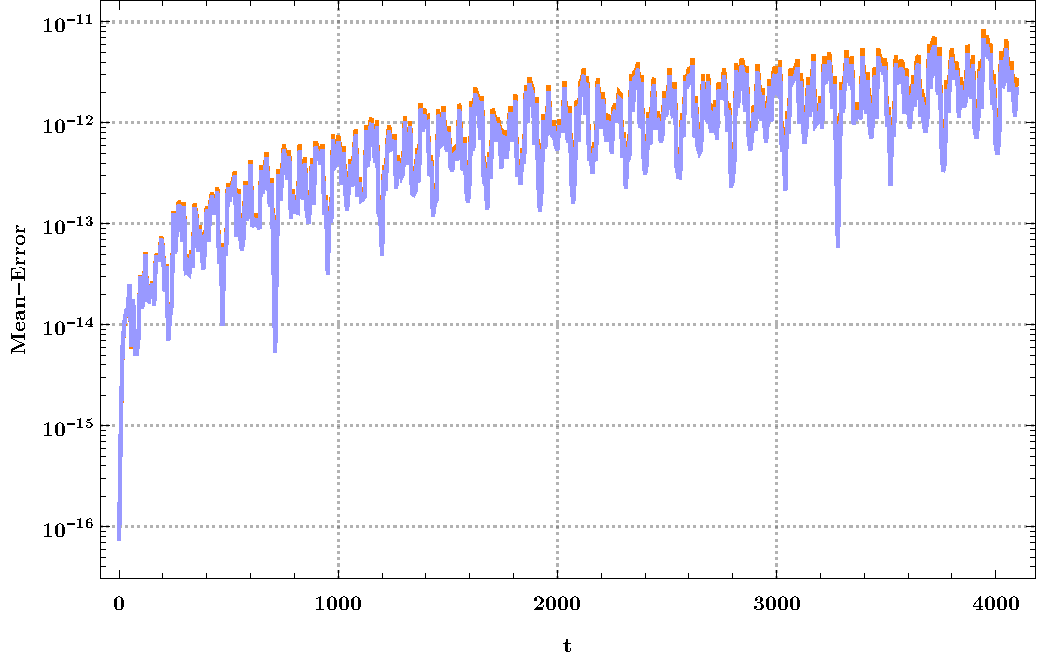
\includegraphics[width=.4\textwidth]{NCDP4A}}
\\
% Zerbitzaria/1-Artikulua-Esperimentuak-4B/13-Esperimentua-V122/Experiments/NCDP-ZAHAR
%
\subfloat[CDP: energy error.]
{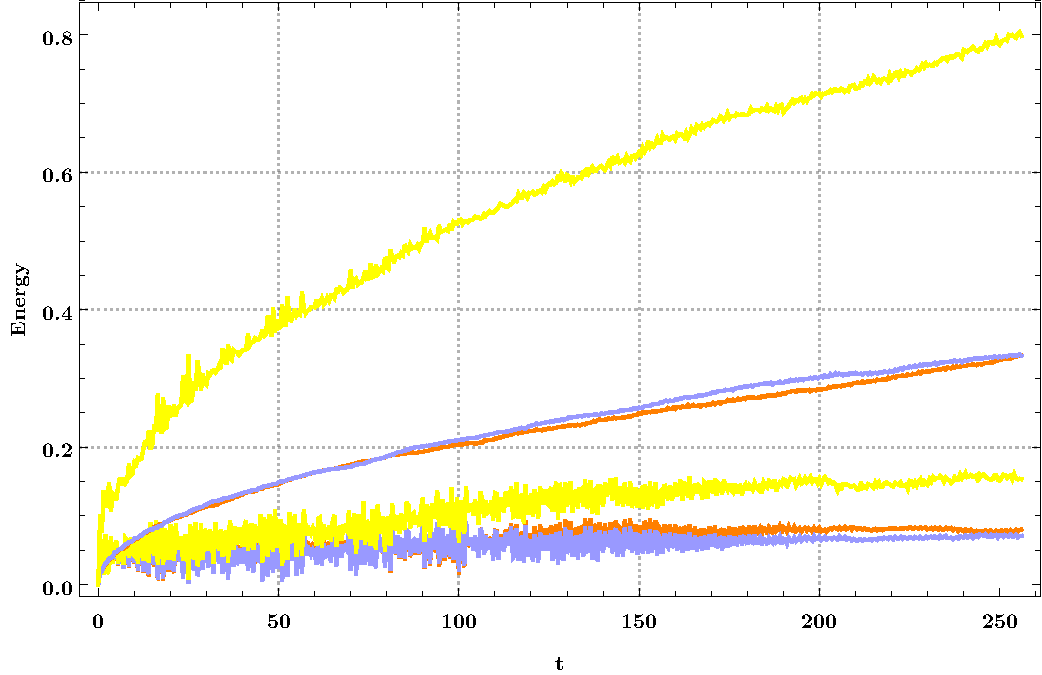
\includegraphics[width=.4\textwidth]{CDP3A}}
&
\subfloat[CDP: mean global error.]
{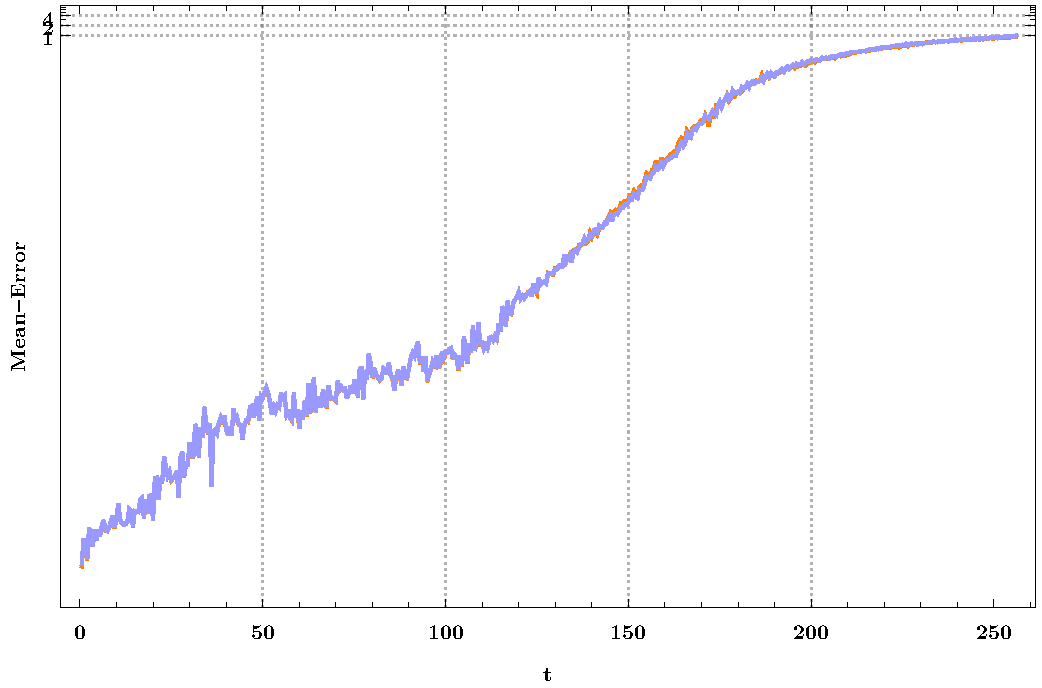
\includegraphics[width=.4\textwidth]{CDP4A}}
% Zerbitzaria/1-Artikulua-Esperimentuak-4B/13-Esperimentua-V122/Experiments
%
\\
\subfloat[6-body: energy error.]
{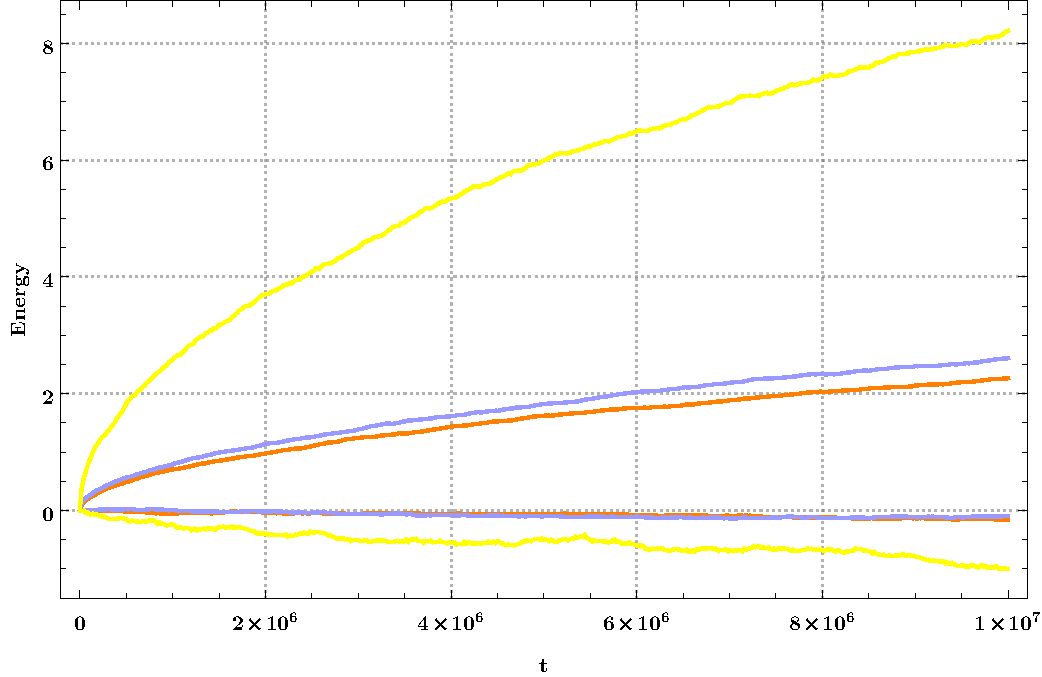
\includegraphics[width=.4\textwidth]{NBODY3A}}
&
\subfloat[6-body: mean global error.]
{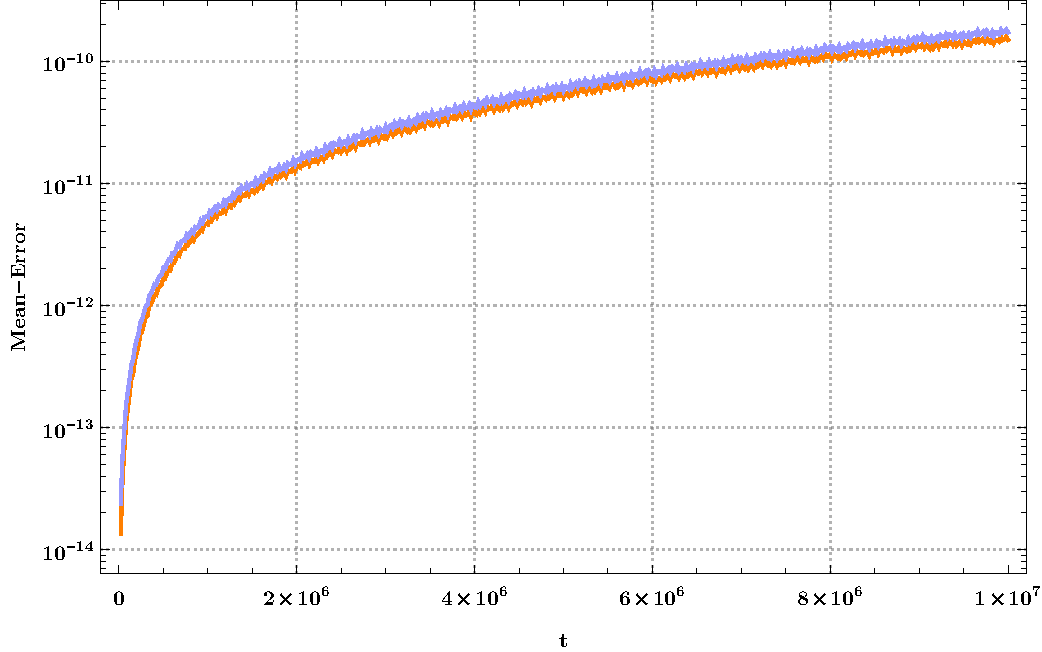
\includegraphics[width=.4\textwidth]{NBODY4A}}
% Zerbitzaria/1-Artikulua-Esperimentuak-4B/13-Esperimentua-V122/Experiments/6-Body (approx=1)
%
\\
\subfloat[10-body: energy error.]
{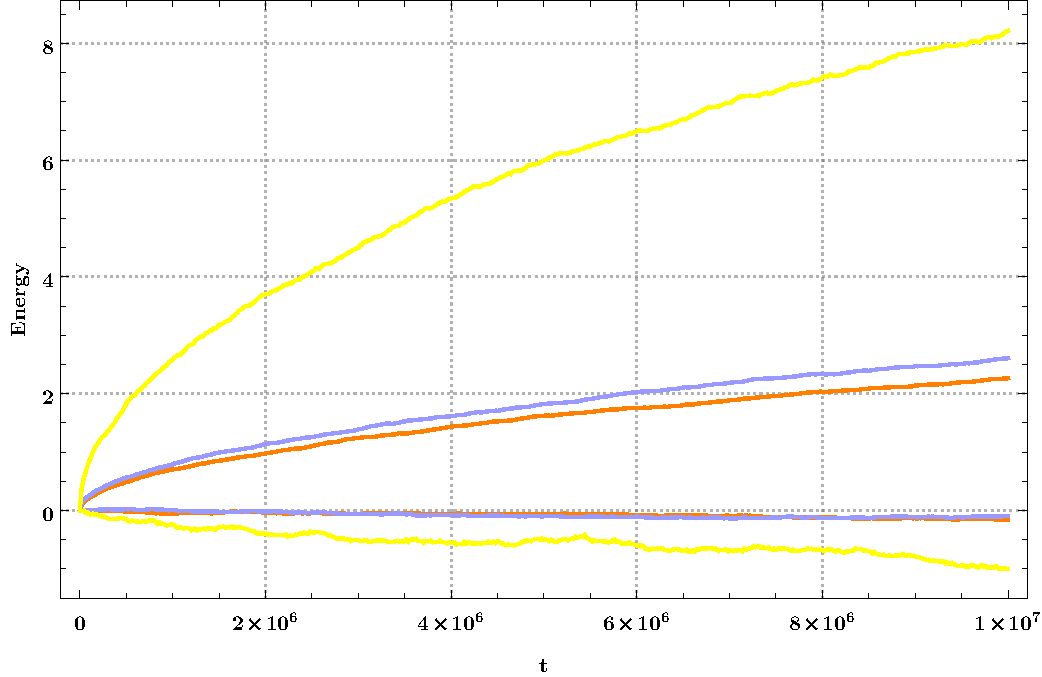
\includegraphics[width=.4\textwidth]{NBODY3A}}
&
\subfloat[10-body: mean global error.]
{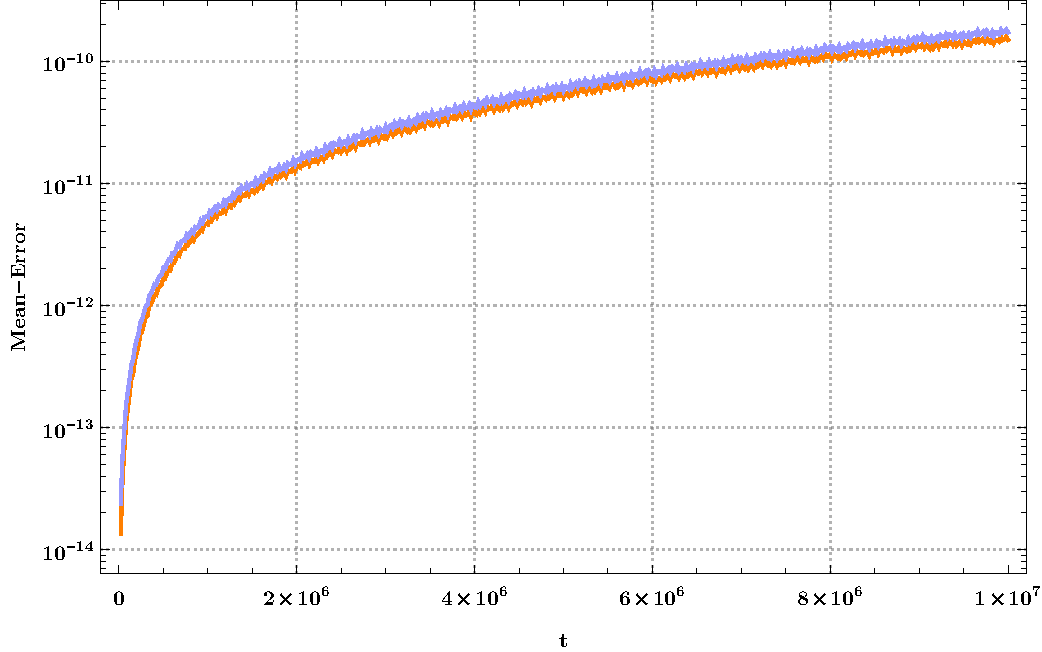
\includegraphics[width=.4\textwidth]{NBODY4A}}
\end{tabular}
\caption{\small Evolution of mean ($\mu$) and standard deviation ($\sigma$) of errors in energy (left) and evolution of Mean of global errors in positions (right), for DP implementation (blue),  FPIEA implementation (orange), and  Hairer's implementation (yellow).  Non-Chaotic case (a,b), Chaotic case (c,d) and outer solar system case (e, f). }
\label{fig:Htt}
\end{figure}

\subsection{Round-off estimation}

\begin{figure}[h]
\centering
\begin{tabular}{c c}
\subfloat[NCDP: original initial values]
{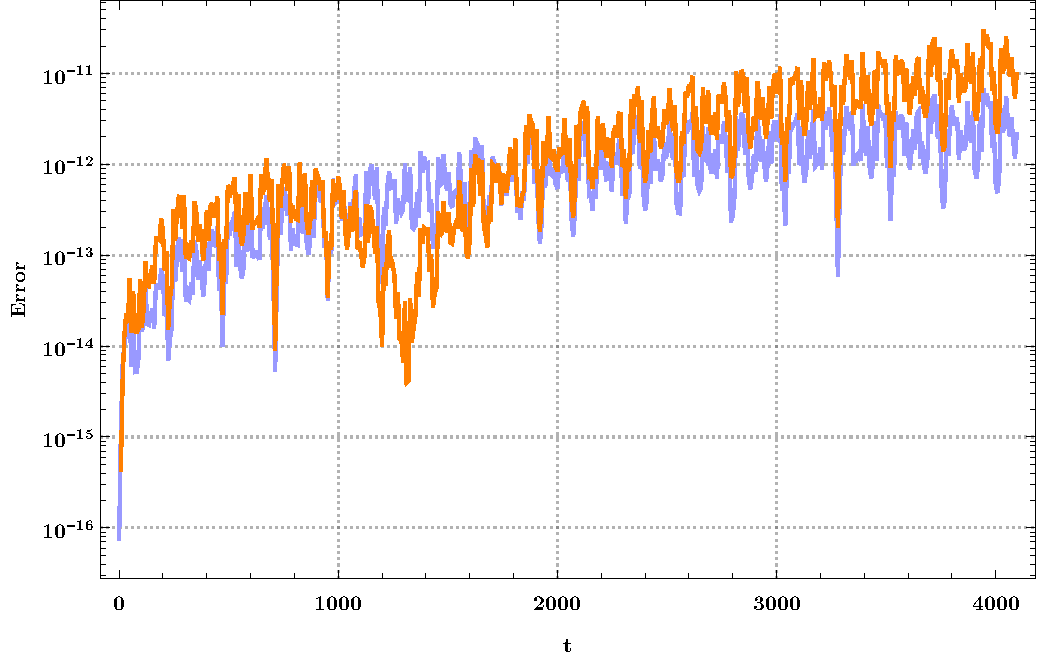
\includegraphics[width=.4\textwidth]{NCDP5A}}
&
\subfloat[NCDP: $P=1000$ perturbed initial values]
{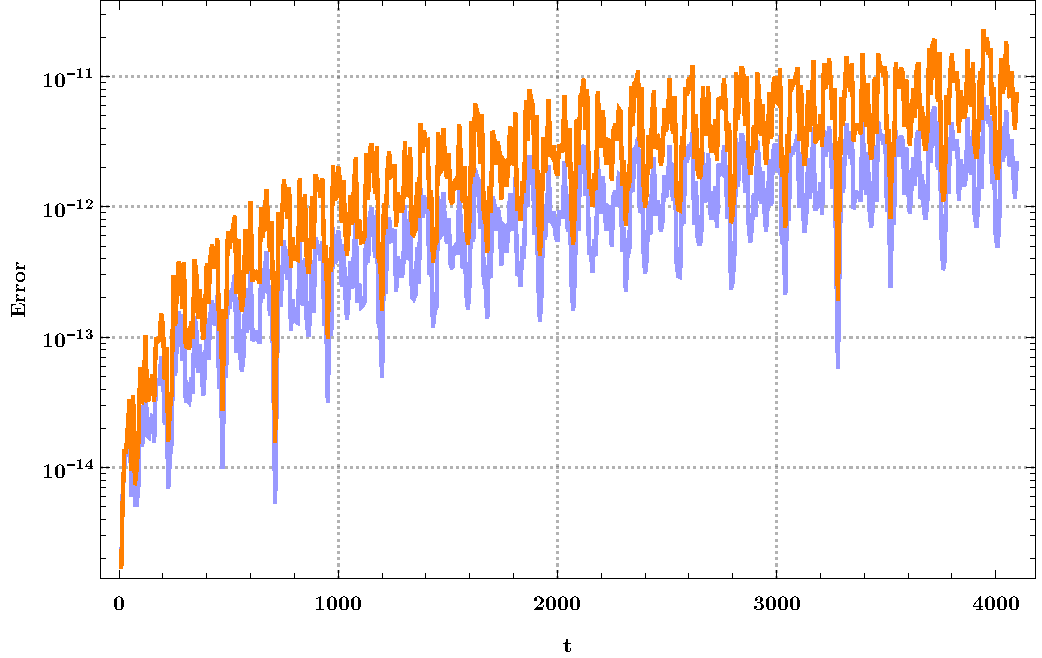
\includegraphics[width=.4\textwidth]{NCDP5B}}
% Zerbitzaria/1-Artikulua-Esperimentuak-4B/13-Esperimentua-V122/Experiments/NCDP-ZAHAR
%
\\
\subfloat[CDP: original initial values]
{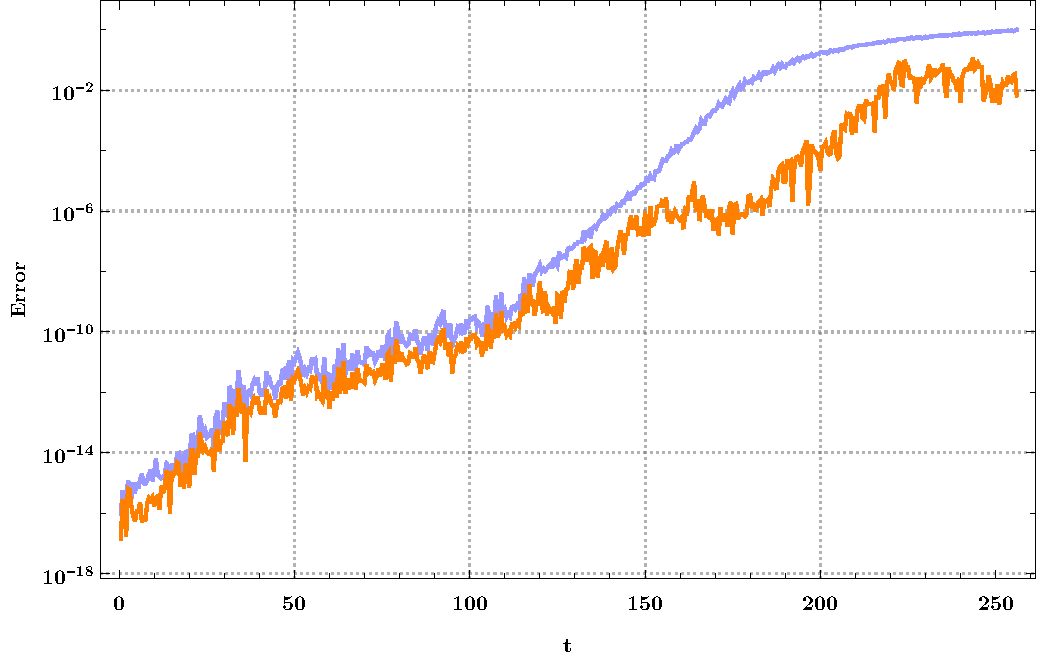
\includegraphics[width=.4\textwidth]{CDP5A}}
&
\subfloat[CDP: $P=1000$ perturbed initial values]
{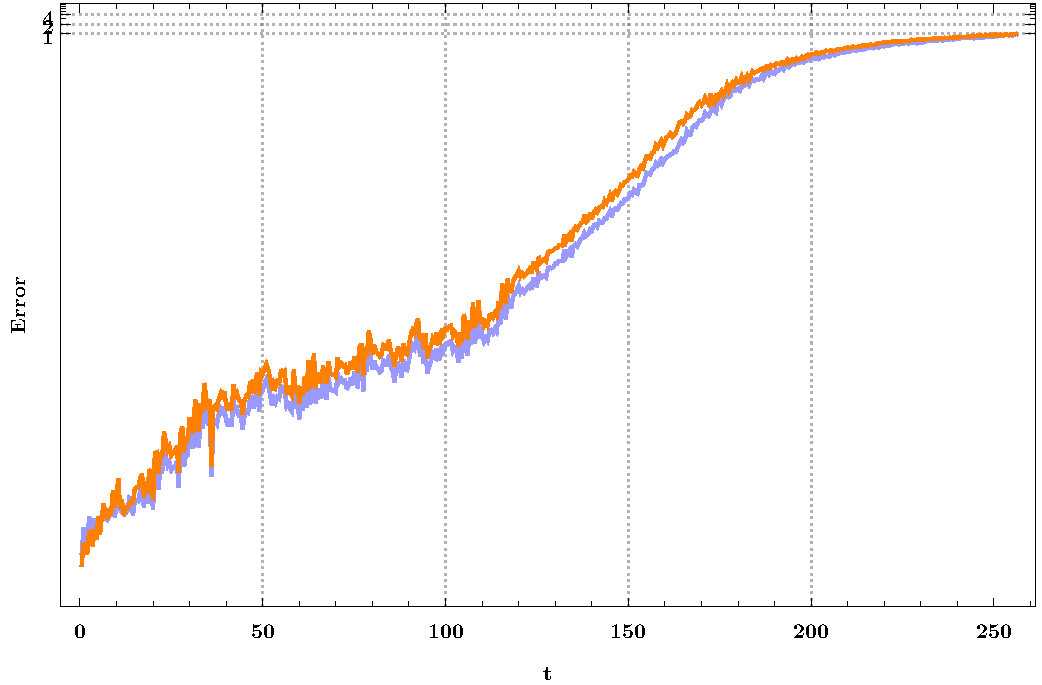
\includegraphics[width=.4\textwidth]{CDP5B}}
% Zerbitzaria/1-Artikulua-Esperimentuak-4B/13-Esperimentua-V122/Experiments
%
\\
\subfloat[6-Body: original initial values]
{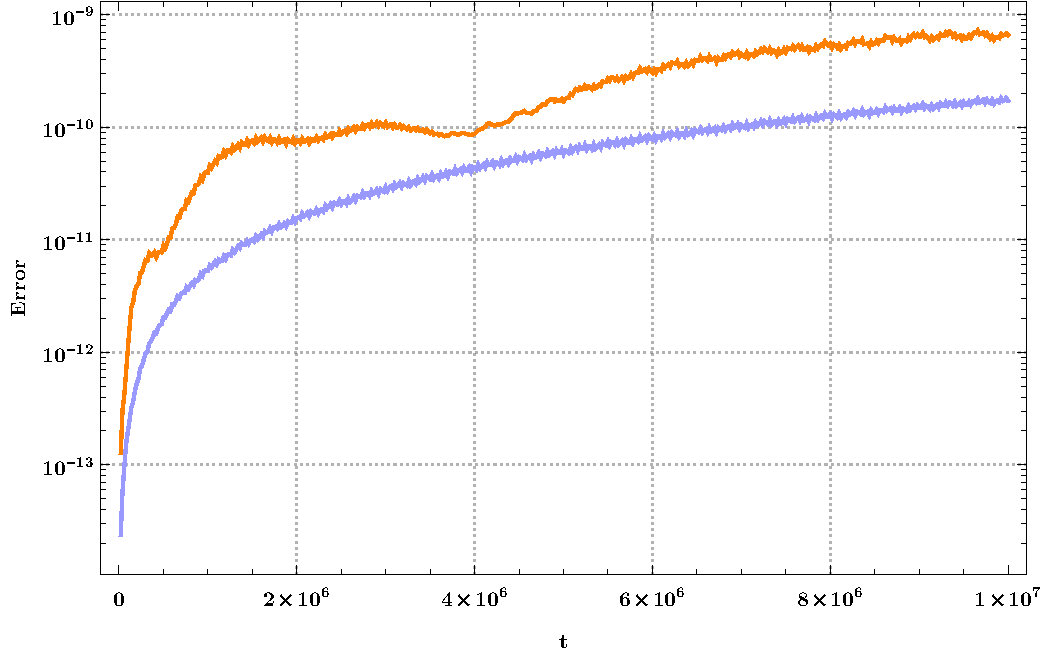
\includegraphics[width=.4\textwidth]{NBODY5A}}
&
\subfloat[6-Body: $P=1000$ perturbed initial values]
{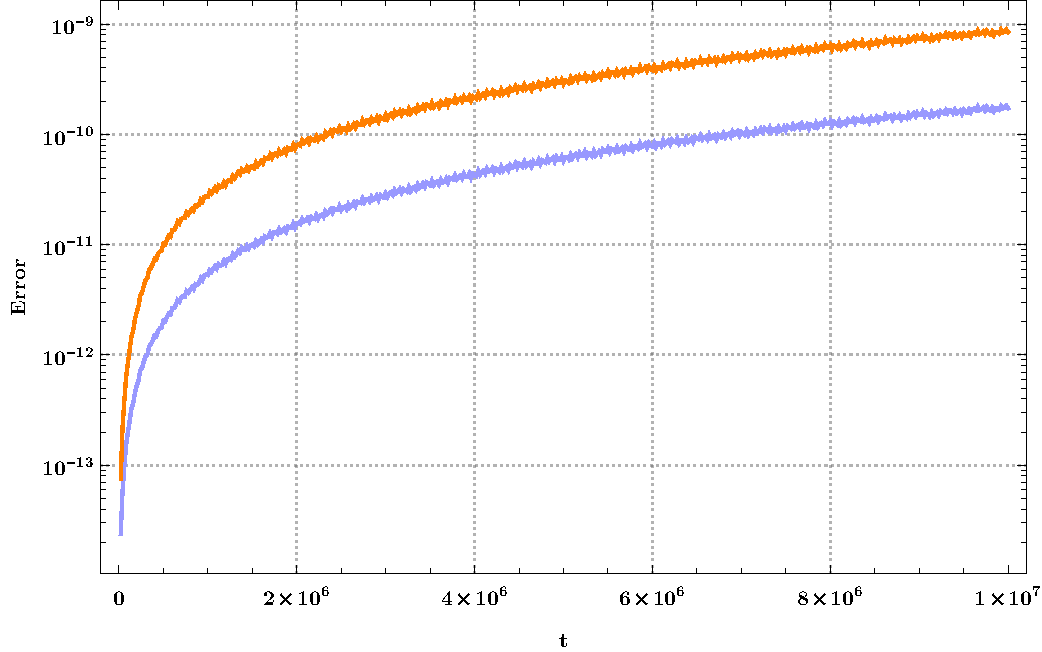
\includegraphics[width=.4\textwidth]{NBODY5B}}
% Zerbitzaria/1-Artikulua-Esperimentuak-4B/13-Esperimentua-V122/Experiments/6-Body (approx=1)
%
\\
\subfloat[10-Body: original initial values]
{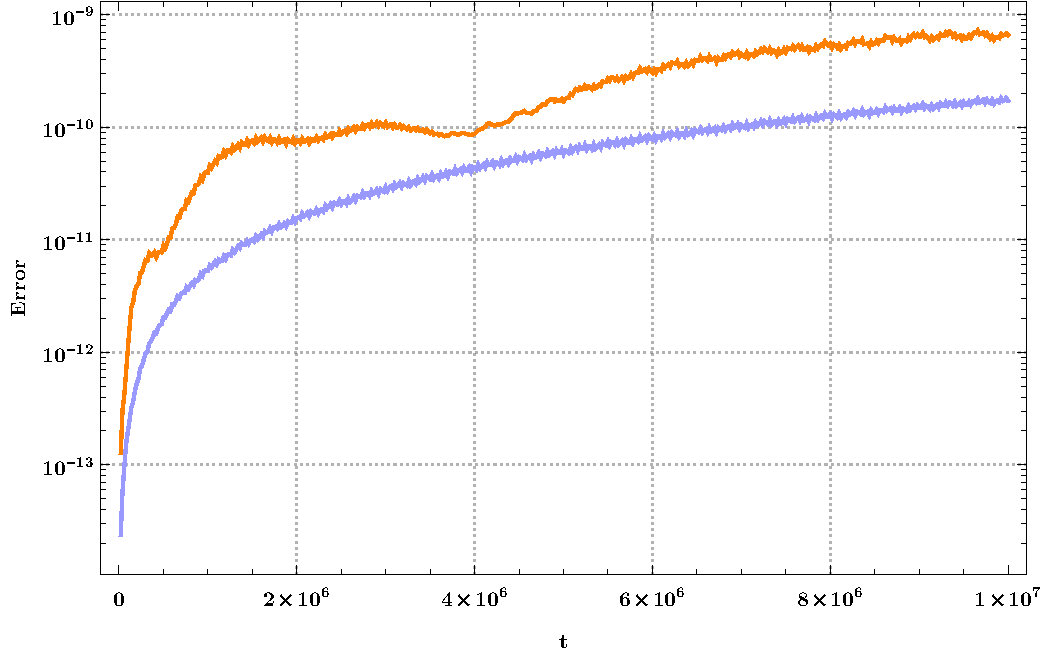
\includegraphics[width=.4\textwidth]{NBODY5A}}
&
\subfloat[10-Body: $P=1000$ perturbed initial values]
{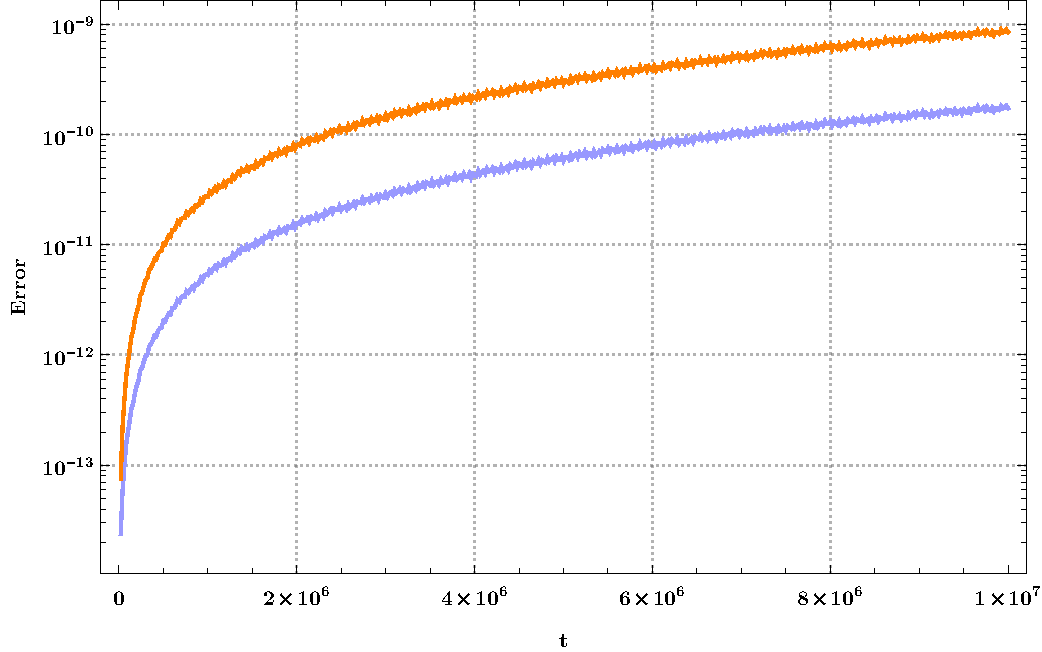
\includegraphics[width=.4\textwidth]{NBODY5B}}
\end{tabular}
\caption{\small Left plots: estimation of the round-off error with the original unperturbed initial values. We compare the evolution of our error estimation (orange) with the evolution of the global error (blue). Right plots:evolution of the mean error in positions (blue) of the application of our DP algorithm to $P=1000$ perturbed initial value problems, together with the evolution of the mean of the estimated errors in positions (orange).}
\label{fig:plot5}
\end{figure}


\clearpage
\section{zaharra}

\subsection{Integrazio motak.}

Erabiltzaileak ekuazio diferentzialaren eskuin aldeko funtzioa, doitasun bikoitzean definituko duela suposatu dugu eta gure inplementazioaren biribiltze errorearen propagazioa idealetik gertu dagoela erakutsi nahi dugu. Gure inplementazioaren zenbakizko soluzioaren $\tilde{y}_n+e_n \approxeq y(t_n) \ (n=1,2,\cdots)$ errorea, jatorri ezberdineko erroreen konbinazioa da. 

\begin{enumerate}

\item Integrazio zehatza.

Konputazio guztia (ekuazio diferentzialaren funtzioaren ebaluazioa barne) doitasun laukoitzeko ($128$-bit) koma higikorreko aritmetikan  egindako integrazioa. Zenbakizko integrazio hau, trunkatze errorea estimatzeko eta errore globala kalkulatzeko erreferentzi gisa (soluzio zehatza) kontsideratuko dugu. 

\item Integrazio superideala.

Zenbakizko integrazio hau iterazio errorea estimatzeko erabiliko dugu. Konputazio guztia doitasun laukoitzean egindako integrazioa baina geratze erizpidea, doitasun bikoitzean neurtuko dugu,
\begin{equation*}
\Delta^{[k]}=|\text{double}(Y^{[k]})-\text{double}(Y^{[k-1]})|.
\end{equation*}

\item Integrazio ideala.

Ekuazio diferentzialaren eskuin aldeko funtzioaren ebaluazioa izan ezik, beste eragiketa guztiak doitasun laukoitzean egiten dituen inplementazioa da. Ekuazio diferentziala doitasun bikoitzean kalkulatzeak, eragiten duen errorea neurtzeko erabiliko dugu eta integrazio hau hobetu ezin daitekeen integrazioa kontsideratuko dugu.   

\item Integrazio sasi-ideala.

Doitasun bikoitzeko koefizienteak ($\tilde{\mu}_ij,\tilde{b}_i$) erabiltzeak eragiten duen errorea neurtzeko integrazioa da. Konputazio guztia doitasun laukoitzean kalkulatzen da baina doitasun bikoitzeko koefizienteen balioak erabiliz (doitasun bikoitzeko koefiziente koadrifikatuak esaten diogu).  
   
\item Double-berria (batura konpensatu hobetua).

Guk proposatutako inplementazioa da. Doitasun bikoitzeko  koma higikorreko aritmetika ($64$-bit) eta gure proposamenak jarraituz inplementatutako \emph{batura konpensatua hobetua} erabiltzen duen inplementazioa, hau da, atalen eguneraketan, ($\tilde{y}_n \oplus \tilde{e}_n$) (ekuazioa \ref{eq:eqbk}) espresioa erabiltzen duen integrazioa.

\item Double-estandarra (batura konpensatu estandarra).

Doitasun bikoitzeko koma higikorreko aritmetika ($64$-bit) eta \emph{batura konpensatu estandarra} erabiltzen duen inplementazioa (atalen eguneraketan $\tilde{e}_n$ gaia kontsideratzen ez duen integrazioa). 

The implementation given in~\cite{Hairer2008}, we will refer to it as Hairer's implementation. We have run their original implicit Runge-Kutta Fortran code  (\href{http://www.unige.ch/~hairer/preprints.html}{Hairer's preprints page}).

\end{enumerate}

Integrazio bakarra egin ordez, ausaz perturbatutako $P=1000$ hasierako balio ezberdinetarako integrazioak exekutatu ditugu eta emaitza hauen guztien batezbestekoan oinarritu gara, biribiltze errorearen azterketa egokia egiteko.    

\subsubsection*{Ausazko perturbazioak.}

Perturbaziorik gabeko hasierako balioa $(u0,e0)$ eta $\mathcal{O}(10^{-6})$ ordeneko $k$ perturbazio tamaina finkatuta, era honetan kalkulatuko dugu $(u1D,e1)$ perturbatutako hasierako balioa,
\begin{lstlisting} [language=Mathematica]
k = 2^(-20);
u1 = u0 + u0*(k*RandomReal[{-1,1}]);
u1D = N[u1];
u1DD = SetPrecision[u1D, prec];
e1 = u1 - u1DD;
\end{lstlisting}

\subsubsection*{Neurtzeko faktoreak.}

Sistema Hamiltondarretan energia kontserbatzen da,
\begin{equation*}
E_i^{[k]}=H(q_i^{[k]}+eq_i^{[k]},p_i^{[k]}+ep_i^{[k]})=konst, \ \ \ i=1,\dots,N/m.
\end{equation*}

\paragraph*{}Energia eta kokapen erroreak honako faktoreen bidez neurtuko ditugu.

\begin{enumerate}

\item Energia errorea.

\begin{align*}
&\Delta E_i^{[k]} =\frac{(E^{[k]}_i-E^{[k]}_0)}{E^{[k]}_0}, \ \ \ i=1,\dots,N/m \ \text{eta} \ k=1,\dots,P.\\
&\bar{\Delta E_i} =\frac{1}{P} \sum_{k=1}^{P} \Delta E_i^{[k]}, \ \  \sigma_i =\sqrt{\frac{1}{P} \sum_{k=1}^{P} (\Delta E_i^{[k]}-\bar{\Delta E_i})^2},\\
&\bar{MaxE } =\max_{i=1,\dots,N} |\bar{\Delta E_i}|.
\end{align*}  

\item Energia diferentzia.

$P$ integrazio baditugu eta $L=N/m$, integrazio bakoitzean lortutako emaitza kopurua bada, $L\cdot P$ balio guztien energiaren diferentzien batezbestekoa ($\bar{\mu}$) eta desbideratze estandarra ($\bar{\sigma}$) kalkulatuko ditugu.            
\begin{align*}
& Dif_i^{[k]} =\frac{(E^{[k]}_i-E^{[k]}_{i-1})}{E^{[k]}_0},\ \ \ i=1,\dots,N/m \ \text{eta} \ k=1,\dots,P, \\
& \bar{\mu} = \frac{1}{L\cdot P} \bigg(\sum_{k=1}^{P} \sum_{i=1}^{L} {Dif_i^{[k]}\bigg)}, \ \
 \bar{\sigma} = \sqrt{\frac{1}{L\cdot P} \bigg(\sum_{k=1}^{P} \sum_{i=1}^{L} {(Dif_i^{[k]}-\bar{\mu)}^2}\bigg)}          
\end{align*}
           
\item Kokapen errore globala.

Doitasun laukoitzean lortutako soluzioa, soluzio zehatza kontsideratuko dugu,           
\begin{equation*}
yexact^{[k]}_i=\hat{y}^{[k]}_i=(\hat{q}^{[k]}_i+\hat{eq}^{[k]}_i,\hat{p}^{[k]}_i+\hat{ep}^{[k]}_i),\ \ i=1,\dots,N/m .
\end{equation*}

eta $k.$ soluzioari ${y}^{[k]}_i=({q}^{[k]}_i+{eq}^{[k]}_i,{p}^{[k]}_i+{ep}^{[k]}_i)$ dagokion kokapen errorea,          
\begin{align*}
&Ge^{[k]}_i =\|(\hat{q}^{[k]}_i+\hat{eq}^{[k]}_i)-(q^{[k]}_i+eq^{[k]}_i)\|_2\\
&\bar{Ge_i} = \left(\frac{1}{P}\sum_{k=1}^{P} Ge^{[k]}_i \right) \ , \
                          \bar{MaxGe}=\max_{i=1,\dots,N/m} (\bar{Ge_i})
\end{align*}     
           
\item Puntu-finkorainoko konbergentzia portzentaien batezbesteko  ($\bar{\Lambda}$).
           
$\Lambda^{[k]}$  $k.$ integrazioan, puntu-finkorainoko konbergentzia lortutako urratsen ehuneko portzentaia izanik,           
\begin{equation*}
\bar{\Lambda}= \frac{1}{p}\sum_{k=1}^{P}\Lambda^{[k]}.
\end{equation*}
 
\item Kokapen errore estimazioa ($\bar{\mu Q_i}$ , $\bar{\sigma Q_i}$). 
            
Biribiltze errorearen estimazioaren gogoratuz, 
\begin{equation}
Est_i^{[k]}=\|(q_i^{[k]}+eq_{i}^{[k]})-(\tilde{\tilde{q}}_i^{[k]}+\tilde{\tilde{eq}}_{i}^{[k]})\|_2
\end{equation}
            
Errore estimazioaren kalitatea neurtzeko,
\begin{align} \label{eq:eq_Qi}
Q_i^{[k]} &=\log_{10} \bigg(\frac{Est^{[k]}_i}{Ge^{[k]}_i}\bigg),\\
\bar{\mu Q_i} &={\frac{1}{P}\sum_{k=1}^{p} Q_i^{[k]}} \ , \ \ 
 \sigma Q_i={\sqrt{\frac{1}{P}\sum_{k=1}^{P} (Q_i^{[k]}-\bar{\mu Q_i})^2}}
\end{align}

\end{enumerate} 


\subsection*{Emaitza nagusiak.}

Esperimentuen emaitzak (\ref{tab:tabDPA}) taula orokorrean eta (\ref{fig:plotDPA}) irudian adierazi ditugu. 

\begin{enumerate}
\item (\ref{tab:tabDPA}) taula orokorra.\\
Taula honetan esperimentuen ikuspegi orokorrena laburtu dugu. Emaitza hauetan, gure inplementazioaren (\emph{Double-berria}) eta \emph{integrazio idealaren} artean diferentzia oso txikia dela baieztatu daiteke. Batetik,  bi integrazioetan energia errorearen eta kokapen errorearen maximoek ia balio berdina hartzen dute. Bestalde, puntu-finkorainoko konbergentzia batezbesteko portzentaia altuak,  urratsa gehienetan puntu-finkoaren iterazioaren bidez lortu daitekeen emaitza hoberena lortzen ari garela adierazten digu.    

\item (\ref{fig:plotDPA}) irudia.
\begin{enumerate}
\item \textbf{(a) irudia: energiaren eboluzioa.}
Irudi honetan \emph{integrazio idealaren}, \emph{Double-berria} eta \emph{Double-estandarra} integrazioak konparatu ditugu. Batetik, espero genuen moduan \emph{Double-berria} integrazioak, \emph{Double-estandarra} integrazioak baino emaitza hobea du. Bigarrenik, \emph{Double-berria} integrazioren eta \emph{integrazio idealaren} energiaren eboluzioak antzekoak dira.

Integrazio mota guztien energiaren batezbestekoaren eboluzioan, drift-a nabarmentzen da. Hurrengo atalean (\ref{Drift}) drift honen jatorria aztertuko dugu.  

\item \textbf{(b) irudia: kokapen errorearen eboluzioa.}
Integrazio tartean zehar, \emph{Double-berri} integrazioaren eta \emph{integrazio idealaren} kokapen errorea parekoak dira (irudian ia ez dira bereizten). Energia errorearekin gertatzen zaigun moduan, \emph{Double-berri} integrazioan kokapen errorea pixka bat handiagoa da. 

\item \textbf{(c) eta (d) irudiak: energia histogramak.}
Energia errorearen ausazkotasuna aztertu dugu. Esperimentu hauetan, $P=1.000$ perturbatutako hasierako balio ezberdinen kopurua bada eta $Nout=512$ integrazio bakoitzean itzulitako diskretizazio kopurua bada, integrazio hauen guztien $521.000$ energia diferentzien laginen histogramak irudikatu ditugu, lagin hauen batezbesteko eta desbideratze estandarreko banaketa normalarekin konparatuz. Bai (\textbf{(c) irudia}) \emph{integrazio idealaren}, bai (\textbf{(d) irudia}) \emph{Double-berri} integrazioaren energia diferentzien laginak bat datoz banaketa normalarekin. 

\item \textbf{(e) eta (d) irudiak: errorearen estimazioa.}     
\textbf{(e) irudian} errorearen estimazioa kokapen errorearekin konparatu dugu: gure estimazioa kokapen errorearen gainetik mantentzen da integrazioan zehar. Estimazioaren kalitatea neurtu dugu \textbf{(d) irudian}:  $0$ eta $2.1$ tartean mantentzen da, eta beraz gehienez estimazioa, kokapen errorea baino bi aldiz handiago da. 

\end{enumerate}

\end{enumerate}
 



\subsubsection*{Energia Drift-a.}
\label{Drift}

(\ref{fig:plotDPA} a) irudian energia batezbestekoak zero izan behar luke integrazio osoan baina drift-a azaldu zaigu. Lehenik, gure inplementazioaren arazoren batek drift hori ez duela sortzen baieztatu behar dugu. Horretarako bi esperimentu berri egin ditugu:

\begin{enumerate}
\item \emph{Integrazio superideala.}
Horretarako, integrazio mota berri bat exekutatu dugu \emph{superideala} deitu duguna: exekuzio osoa doitasun laukoitzean baina geratze irizpidea \emph{double moduan} aplikatua,
\begin{equation*}
\Delta =\|Double(Y^{[k]})-Double(Y^{[k-1]})\|.
\end{equation*}
\emph{Integrazio superidealaren} emaitzak (\ref{fig:plotDrift}(a) irudia) ikus daitezke eta bertan, \emph{superideala integrazioak} ere energia drift-a azaltzen duela ikusi daiteke.

\item Hairer-en inplementazioaren azterketa. Hairer-ek bere lanean \cite{Hairer2008} bi problema (Hénon-Helies eta kanpo eguzki-sistema) aztertu zituen eta energia dirft-aren arazoa konpondutzat eman zuen. Guk Hairer-en kodearekin Pendulu bikoitzaren problema integratu dugu eta bere inplementazioan ere, energiaren drift-a badagoela baieztatu dugu. Hala ere,  \ref{fig:plotDrift}(b) irudian energia drift-a gure inplementazioa baino txikiago duela adierazi behar dugu.

\end{enumerate}


\begin{figure}[!h]
\centering
\subfloat[Energi drift: gure inplementazioa]{
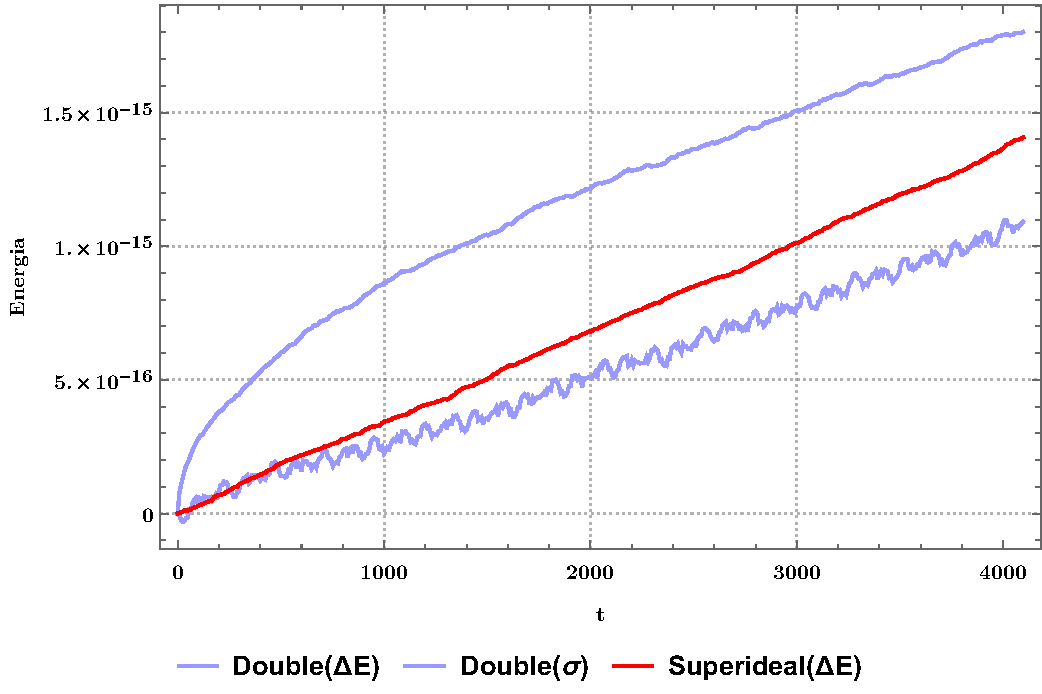
\includegraphics[width=.500\textwidth]{plotSuperIdeala}
}
\subfloat[Energi drift: Hairer-en inplementazioa]{
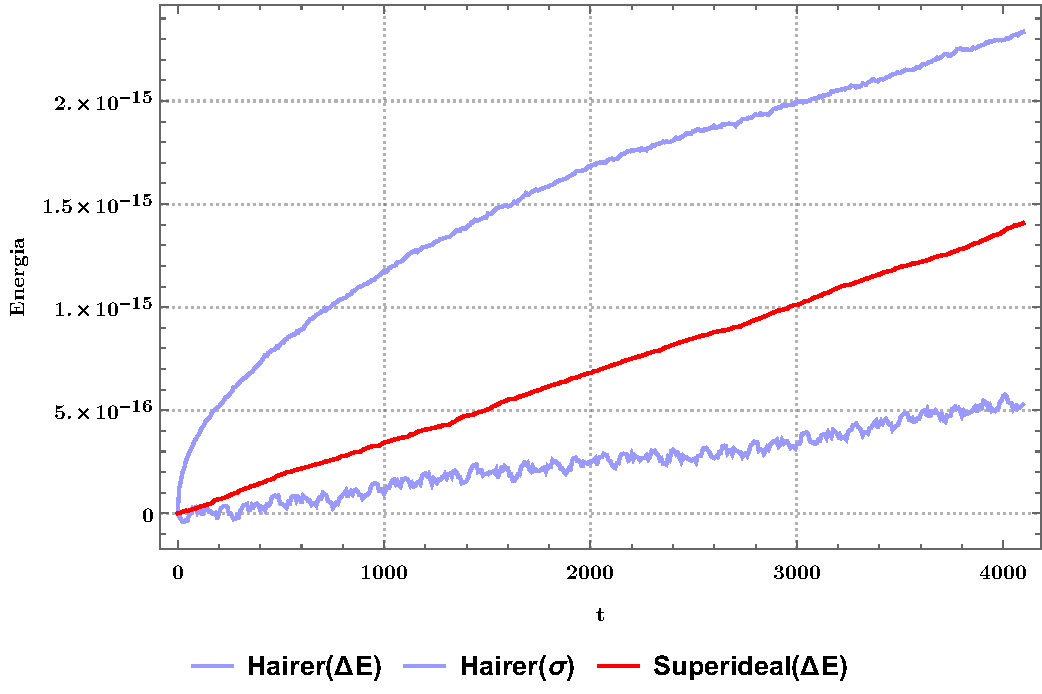
\includegraphics[width=.500\textwidth]{plotHairer}
}
\caption[Energi drift-a (I).]
        {\small Energia Drift-a (I) (Pendulu-bikoitza ez-kaotikoa).
        
         \textbf{(a) irudian}, gure inplementazioaren emaitzak ikusi daitezke: \emph{superidealaren} integrazio bakarraren energia errore erlatiboa  eta \emph{Double-Berri} bertsioaren $P=1.000$ integrazioen energia batezbestekoa eta desbideratze estandarra. 
%
%        05-09-2016: Esperimentua errepasatu.
%          SuperIdeala berriz exekutatu ?         
%          (/C-inplementazioa/Code-bertsioak/41-Bertsioa/Experiments/DoublePendulum(NonChaotic)V3).
%          (/C-inplementazioa/Code-bertsioak/41-Bertsioa/Experiments/DoublePendulum(NonChaotic)V9..Tesirako irudiak).
                 
         \textbf{(b) irudian}, Hairer-en inplementazioaren $p=1000$ integrazioen energia batezbestekoa eta desbideratze estandarra , gure inplementazioaren \emph{superidealaren} integrazio bakarraren energia errore erlatiboarekin konparatu ditugu.
         
%        /4-Hairer IRK (Fortran)/1-Hairer-IRK(Double Pendulum)/Experiment/1-Double PendulumV9 ... Tesi irudiak
%        
}
\label{fig:plotDrift}
\end{figure}        


Bigarrenik, energiaren drift-aren arrazoia bilatu nahi dugu. Gure ustez, energiaren drift-aren jatorria, puntu-finkoaren iterazioen erroreak eragindakoa da: puntu-finkoaren iterazioen konbergentzia $O(h)$ da. Zentzu honetan bi esperimentu berri egin ditugu: 

\begin{enumerate}
\item Newton sinplifikatua. 
Newton sinplifikatuaren iterazioen konbergentzia $O(h^2)$ da. Newton sinplifikatuan oinarritutako inplementazio berri batekin Pendulu bikoitzaren integrazioa errepikatu dugu eta energiaren drift-a ez dagoela baieztatu dugu (ikus \ref{fig:plotDrift2} (a) irudia). Beraz, puntu-finkoaren metodoak berezkoa duen errorea kontsidera daiteke.

\item Sasi-Newton.
 Hala ere, azken urratsa bezala, LU-deskonposaketa eragiketa eta jakobiarra  behar ez duen inplementazio eskaini nahi diogu erabiltzaileari. Esperimentalki frogatu dugu modu honetan ere, energiaren drift-a desagertu dela (ikus \ref{fig:plotDrift2} (b) irudia).
 
Jarraian, IRK puntu-finkoaren eta Newton Sinplifikatuaren arteko algoritmoa azalduko dugu. Newton metodo sinplifikatua, $k=1,2,\dots$  $L_i^{[k]}$ hurbilpenak kalkulatzeko algoritmoa hau bada,
\begin{enumerate}
\item 
$g_i^{[k]}=-L_i^{[k-1]}+h b_i f(t+c_ih,y_n+ \sum\limits_{j=1}^{s} \mu_{ij} L_{j}^{[k-1]}), \ \ i=1,\dots,s.$

\item Solve $\Delta L_i^{[k]}$,

$\Delta L_i^{[k]} - h b_i \sum_{j=1}^{s} \mu_{ij} \ J_j \ \Delta L_j^{[k]} = g_i^{[k]}  , \ \ i=1,\dots,s.$

\item $L_i^{[k]} = L_i^{[k-1]}+ \Delta L_i^{[k]}, \ \  i=1,\dots,s.$

\end{enumerate}

Modu merkean, $\Delta L_i^{[k]}$ era honetan hurbildu daiteke,  
\begin{align*}
\Delta L_i^{[k]}= \frac{h b_i}{\lambda} \bigg(f(Y_{i}^{[k]}+ \sum_{j=1}^{s} \lambda \mu_{ij} g_j^{[k]})-f(Y_{i}^{[k]}) \bigg)
\end{align*}
non $\lambda=2^{10}$.

\end{enumerate}

%\begin{align*}
%R_{n,i}^{[k]}&=hb_i \ f(Y_{n,i}^{[k]})-L_{n,i}^{[k]} \\
%\Delta L_{n,i}^{[k]}&=R_{n,i}^{[k]}+hb_i \ f'(Y_{n,i}^{[k]}) \ \sum\limits_{j=1}^{s} \mu_{ij} \Delta L_{n,i}^{[k]} \\
%L_{n,i}^{[k+1]}&=L_{n,i}+\Delta L_{n,i}^{[k]}
%\end{align*}

%\begin{align*}
%R_{n,i}^{[k]}&=hb_i \ f(Y_{n,i}^{[k]})-L_{n,i}^{[k]} \\
%\Delta L_{n,i}^{[k]}&=R_{n,i}^{[k]}+\frac{hb_i}{\lambda} \big(f(Y_{n,i}^{[k]}+\sum\limits_{j=1}^{s} \lambda \mu_{ij} \ %R_{n,i}^{[k]})-f(Y_{n,i}^{[k]}) \big) \\
%L_{n,i}^{[k+1]}&=L_{n,i}+\Delta L_{n,i}^{[k]}
%\end{align*}
%non $\lambda=2^{10}$.

\begin{figure}[!h]
\centering
\subfloat[Newton sinplfikatua]{
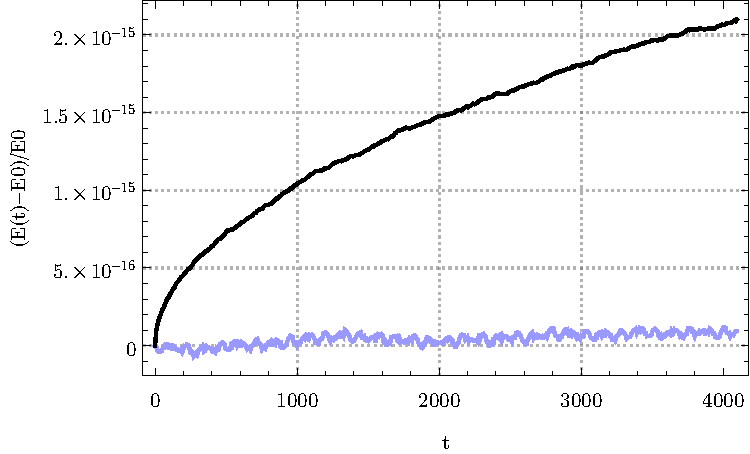
\includegraphics[width=.500\textwidth]{plotNewtonDP}
}
\subfloat[SasiNewton]{
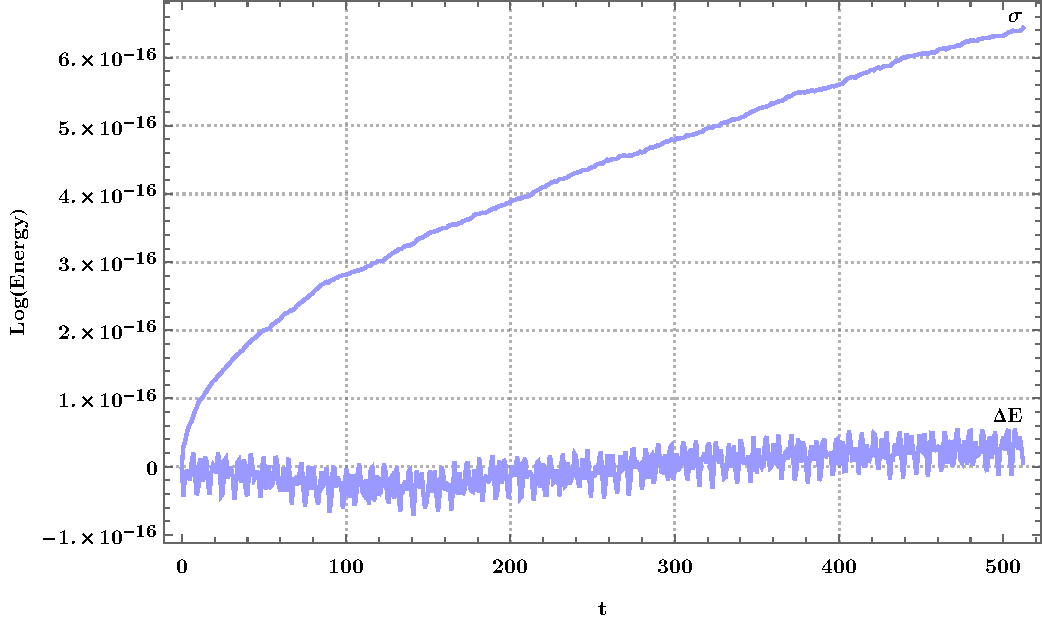
\includegraphics[width=.500\textwidth]{SasiNewton}
}
\caption[Energi drift-a (II).]
        {\small Energia Drift-a (II) (Pendulu-bikoitza ez-kaotikoa).
        
        \textbf{(a) irudian } puntu-finkoaren iterazioaren ordez Newton sinplifikatua aplikatuz integrazioen energia batezbestekoa eta desbideratze estandarra.      
%        Kodea: /61-Newton Sinplifikatua/C-inplementazioa/Code-Bertsioak/2-Bertsioa/Experiments/NonChaoticDouble-3/
%                Exekuzioa: Zerbitzaria/1-Artikulu-Esp-12(Newton)/Experiments/NonChaoticDouble-2

        \textbf{(b) irudian }, puntu-finkoaren iterazioaren ordez SasiNewton aplikatuz integrazioen energia energiaren errorearen batezbestekoa eta desbideratze estandarra. Esperimentu honetan integrazio tarte txikiagoa exekutatu dugu ($t=2^9$).       
%        SasiNewton.Nire portatilean exekuzioa. /1-IRK Kodeak/61-Newton  Sinplifikatua/C-inplementazioa/Code-Bertsioak/3-Bertsioa (Beta)/Experiments/NonChaoticDouble-2   
}
\label{fig:plotDrift2}
\end{figure}   

    
\clearpage


\subsubsection*{Emaitza nagusiak.}

Esperimentuen emaitzak (\ref{tab:tabDPB}) taulan eta (\ref{fig:plotDPB}) irudian adierazi ditugu. Problema kaotikoa denez, kokapen errorea esponentzialki handitzen da eta horregatik integrazio tarte txikiagoa aukeratu da. Orokorrean, Pendulu bikoitza ez-kaotikoaren esperimentuen ezaugarriak mantentzen dira. Esan, esperimentu hauetan ez dela energia drift-arik azaltzen (integrazio tartea txikia delako) eta energia diferentzien histogramak ez datozela erabat dagokion banaketa normalarekin. 

\begin{table} [h]
\caption{Pendulu Bikoitza kaotikoaren laburpena.}
\label{tab:tabDPB}       % Give a unique label
\begin{tabular}{c|c c c c c} 
 Arithmetic   &  $\bar{\Lambda}$  &  $\bar{MaxE}$ & $\bar{\mu}$  & $\bar{\sigma}$   & $\bar{MaxGe}$  \\
                           &   \%            &       &          &            &         \\
 \hline
                         &                 &         &       &             \\
 Zehatza                 &   $94$          &  $2e10^{-19}$  & $4e10^{-22}$  & $9e10^{-21}$   &          \\	    
 Ideala                  &   $98$          &  $8e10^{-17}$  & $1e10^{-19}$  & $3e10^{-17}$   & $0.33$   \\
 Double-berria           &   $95$          &  $8e10^{-17}$  & $1e10^{-19}$  & $3e10^{-17}$   & $0.34$   \\
 Double-estandarra       &   $95$          &  $9e10^{-17}$  & $1e10^{-19}$  & $3e10^{-17}$   & $0.35$   \\
\end{tabular}
\end{table}

\begin{figure}[!h]
\centering
\subfloat[Energi errorea.]{
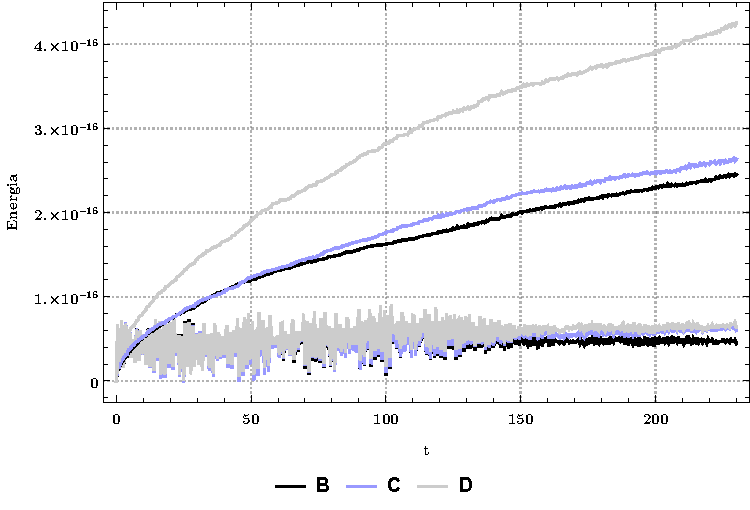
\includegraphics[width=.500\textwidth]{DPBplot1}
%plot3c-2
}
\subfloat[Kokapen errorea.]{
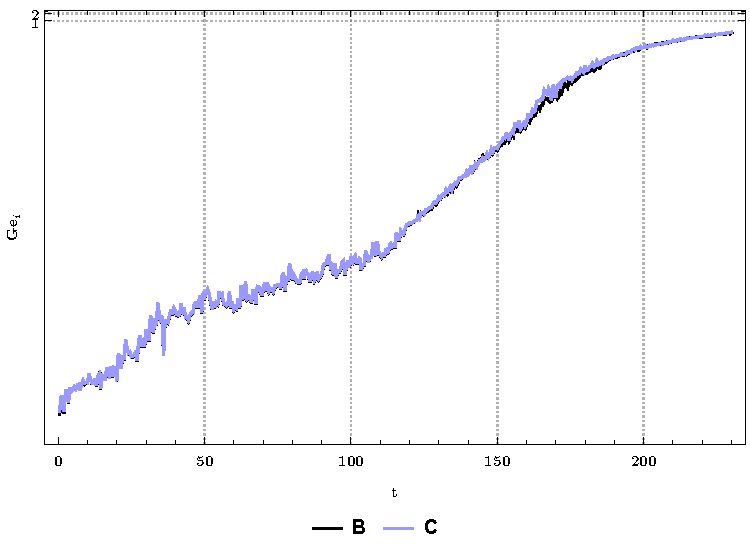
\includegraphics[width=.500\textwidth]{DPBplot3}
%plot3d
}
\vskip\baselineskip
\subfloat[Histograma ideala.]{
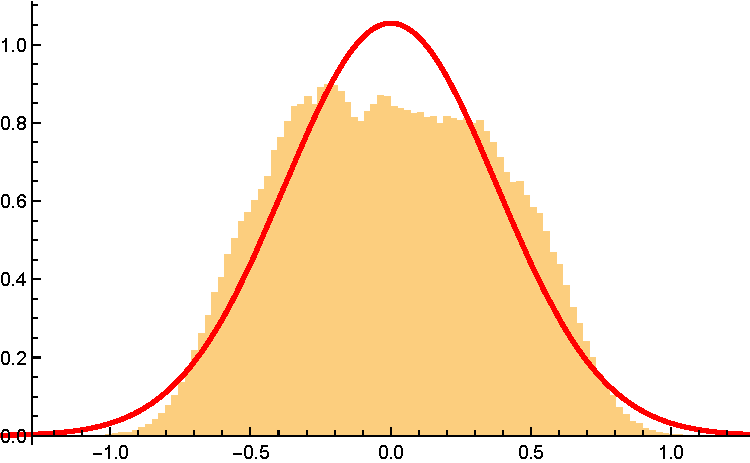
\includegraphics[width=.450\textwidth]{DPBplot4}
%brouwer4c
}
\subfloat[Histograma Double-berri.]{
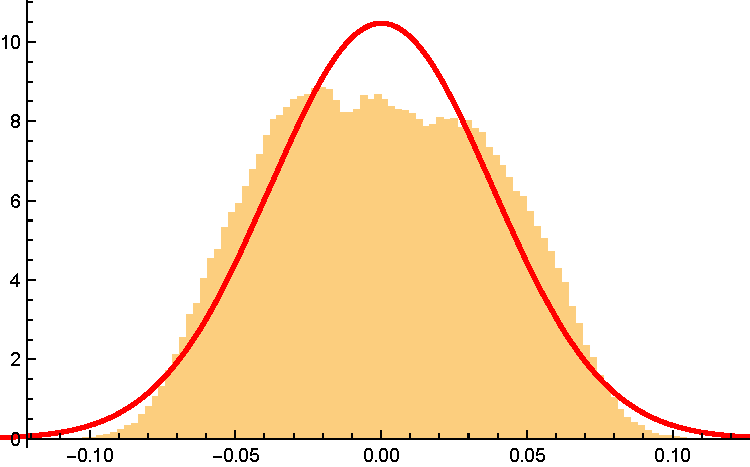
\includegraphics[width=.450\textwidth]{DPBplot5}
%brouwer4d
}
\vskip\baselineskip
\subfloat[Errore estimazioa]{
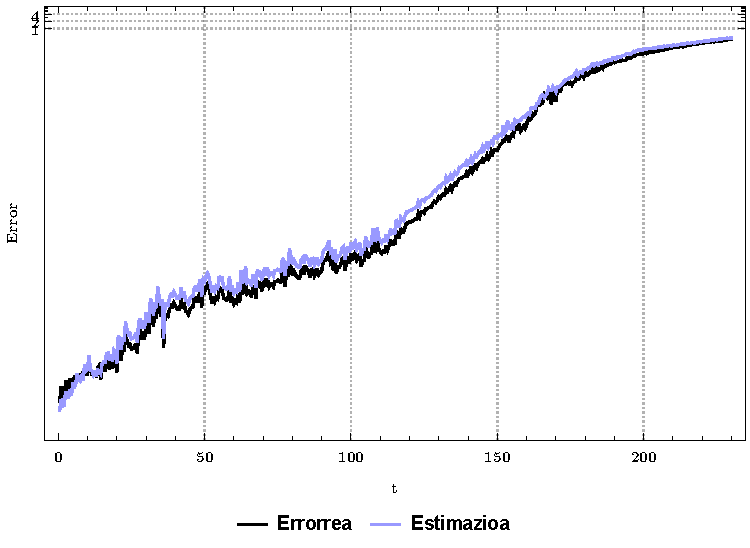
\includegraphics[width=.500\textwidth]{DPBplot6}
%plot5c
}
\subfloat[Errore estimazioaren kalitatea]{
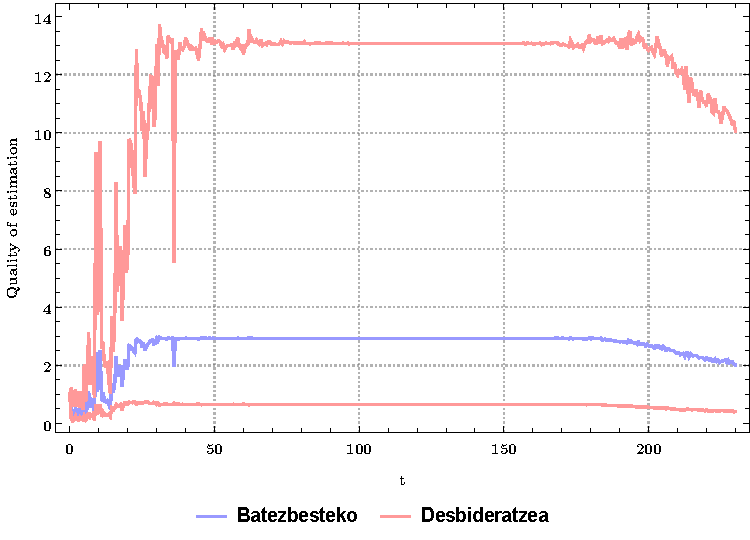
\includegraphics[width=.500\textwidth]{DPBplot7}
%plot5d 
}
\caption[Pendulu-bikoitza: kaotikoa.]
        {\small Pendulu-bikoitza kaotikoa.
        
         \textbf{(a) irudian},  energi errorearen batezbestekoaren ($\bar{\Delta E_i}$) eta  desbideratze estandarraren ($\sigma_i$) eboluzioa. \textbf{(b) irudian}, kokapen errorearen eboluzioa $\bar{Ge_i}$. Honako laburdurak erabili ditugu: B=Integrazio ideala, C=Double-Berria, D=Double-estandarra.
                
                 \textbf{(c) eta (d) iruditan} $P=1.000$ integrazio ezberdinen $521.000$ energi diferentzien laginen histogramak irudikatu ditugu, batezbesteko eta desbideratze estandar bereko banaketa normalarekin alderatuz.Ardatza horizontalak $10^{-16}$ unitatea adierazten du.
                
                 \textbf{(e) irudian} errorearen estimazio kokapen errorearekin konparatu dugu. \textbf{(f) irudian} estimazioaren kalitatea aztertu dugu: (\ref{eq:eq_Qi}) definizioaren arabera, estimazio-kalitatearen batezbestekoa $\bar{\mu Q_i}$  eta desbideratze estandarra $\bar{\sigma Q_i}$ irudikatu ditugu.        
        }
\label{fig:plotDPB}
\end{figure}  

\clearpage
\subsection{N-Body problema.}

Problema honetan erabilitako integrazio tartea eta urratsa luzera hauek izan dira,
\begin{align*}
& t_0=0, \ \ t_{end}=10^{6}, \\
& h=2, \\
& sampling=1000, step=1.\\
& P=1.000, \ N=500. 
\end{align*} 

(integrazioen iraupena=$xx$ egun).

Esperimentuen emaitzak (\ref{tab:tabNBODY}) taulan eta (\ref{fig:plotNBODY}) irudian adierazi ditugu. Azpimarratu nahi dugu N-Body probleman ez zaigula energia Drift-arik agertu. N-Body problema bigarren ordeneko ekuazio diferentzial arrunta da eta \emph{Gauss-Seidel} moduko iterazioa aplikatu dugu (konbergentzia azkarragoa).

\begin{table} [h]
\caption{N-Body problemaren laburpena.}
\label{tab:tabNBODY}       % Give a unique label
\begin{tabular}{c|c c c c c} 
 Arithmetic   &  $\bar{\Lambda}$  &  $\bar{MaxE}$ & $\bar{\mu}$  & $\bar{\sigma}$   & $\bar{MaxGe}$  \\
                           &   \%            &       &          &            &         \\
 \hline
                           &                 &         &       &           &          \\
 Zehatza                   &   $98.$        &  $2e10^{-19}$  & $5e10^{-24}$  & $2e10^{-20}$  &      \\	    
 Ideala                    &   $99.$        &  $6e10^{-18}$  & $6e10^{-21}$  & $3e10^{-19}$ &  $7e10^{-12}$\\
 Double-berria             &   $98.$       &  $5e10^{-18}$  & $4e10^{-21}$  & $3e10^{-19}$ &  $1e10^{-11}$\\
 Double-estandarra         &   $98.$       &  $5e10^{-18}$  & $4e10^{-21}$  & $3e10^{-19}$ &  $1e10^{-11}$\\
\end{tabular}
\end{table}


\begin{figure}[!h]
\centering
\subfloat[Energi errorea.]{
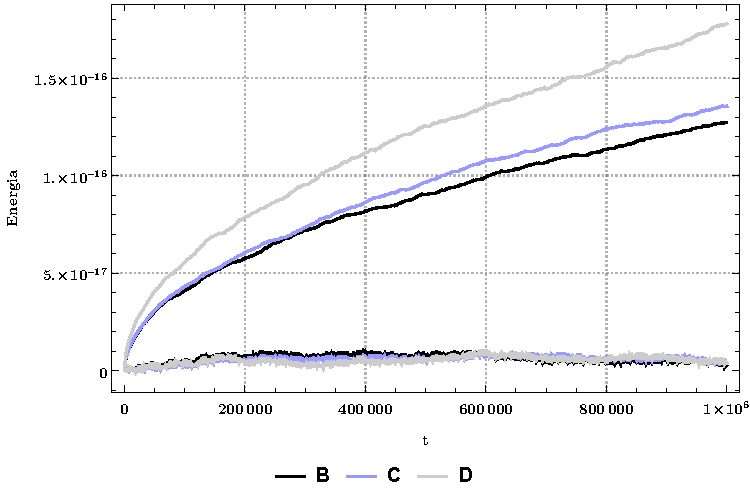
\includegraphics[width=.500\textwidth]
{NBODYplot1}
%{plot6a}
}
\subfloat[Kokapen errorea.]{
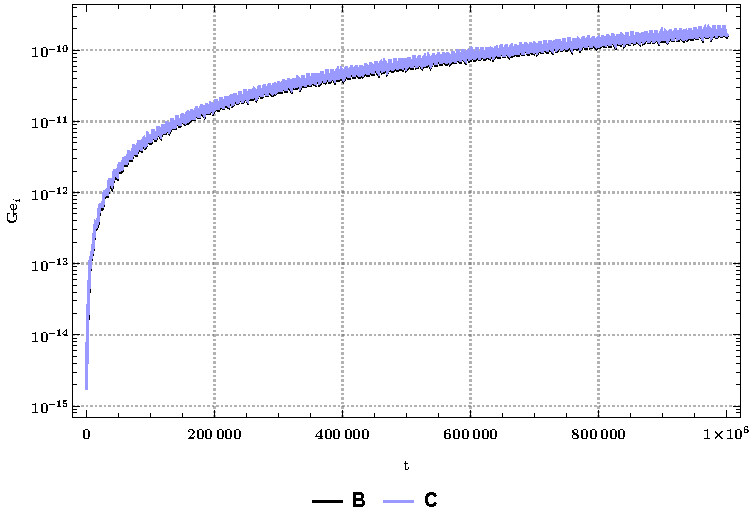
\includegraphics[width=.500\textwidth]
{NBODYplot3}
%{plot6b}
}
\vskip\baselineskip
\subfloat[Histograma ideala.]{
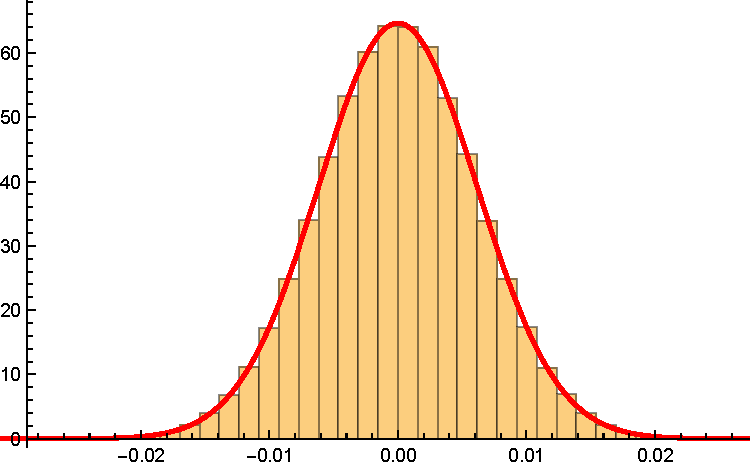
\includegraphics[width=.450\textwidth]
{NBODYplot4}
%{brouwer4e}
}
\subfloat[Histograma Double-berri.]{
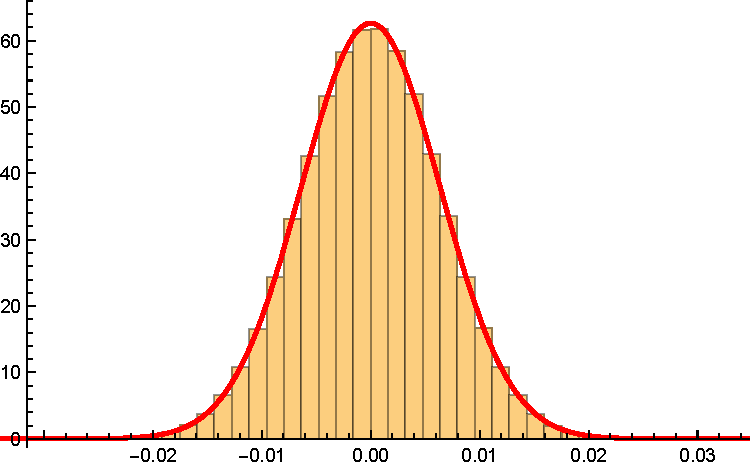
\includegraphics[width=.450\textwidth]
{NBODYplot5}
%{brouwer4f}
}
\vskip\baselineskip
\subfloat[Errore estimazioa]{
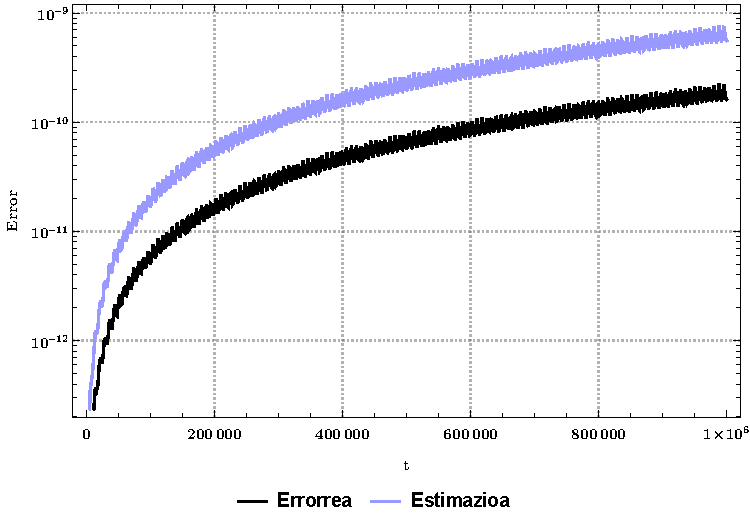
\includegraphics[width=.500\textwidth]
{NBODYplot6}
%{plot7a}
}
\subfloat[Errore estimazioaren kalitatea]{
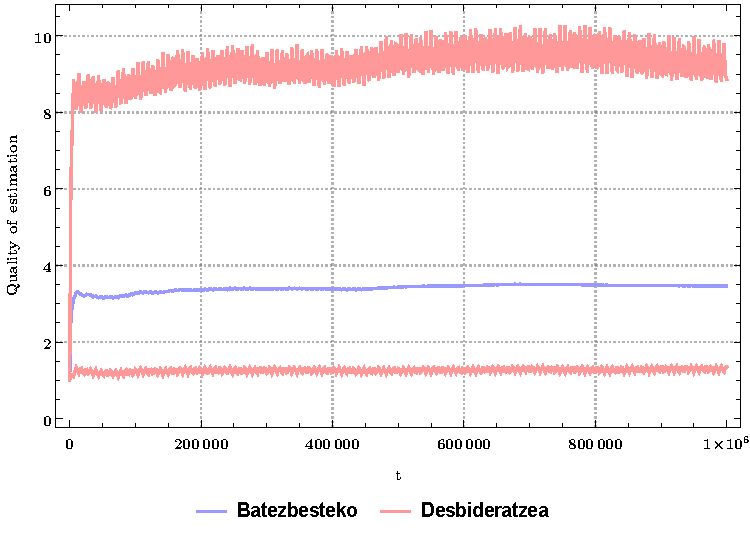
\includegraphics[width=.500\textwidth]
{NBODYplot7} 
%{plot7b}
}
\caption[N-Body.]
        {\small N-Body.
        
         \textbf{(a) irudian},  energi errorearen batezbestekoaren ($\bar{\Delta E_i}$) eta  desbideratze estandarraren ($\sigma_i$) eboluzioa. \textbf{(b) irudian}, kokapen errorearen eboluzioa $\bar{Ge_i}$. Honako laburdurak erabili ditugu: B=Integrazio ideala, C=Double-Berria, D=Double-estandarra.
                
                 \textbf{(c) eta (d) iruditan} $P=1.000$ integrazio ezberdinen $521.000$ energi diferentzien laginen histogramak irudikatu ditugu, batezbesteko eta desbideratze estandar bereko banaketa normalarekin alderatuz.Ardatza horizontalak $10^{-16}$ unitatea adierazten du.
                
                 \textbf{(e) irudian} errorearen estimazio kokapen errorearekin konparatu dugu. \textbf{(f) irudian} estimazioaren kalitatea aztertu dugu: (\ref{eq:eq_Qi}) definizioaren arabera, estimazio-kalitatearen batezbestekoa $\bar{\mu Q_i}$  eta desbideratze estandarra $\bar{\sigma Q_i}$ irudikatu ditugu.        
        }
\label{fig:plotNBODY}
\end{figure}      

\subsubsection*{Momentu angeluarra.}

N-Body probleman momentu angeluarra,
\begin{equation*}
O=\sum_{i=0}^{N} \mathbf{p_i} \times \mathbf{q_i}.
\end{equation*}
metodo sinplektikoek mantentzen duten inbariantea da. Hurrengo grafikoetan (irudia \ref{fig:plotNBODYMOM}) horrela baieztatu daiteke.

\begin{figure}[!h]
\centering
\subfloat[Momentu angeluarra(Lx).]{
\includegraphics[width=.500\textwidth]
{NBODYplot21}
}
\subfloat[Momentu angeluarra(Ly).]{
\includegraphics[width=.500\textwidth]
{NBODYplot22}
}
\vskip\baselineskip
\subfloat[Momentu angeluarra(Lz).]{
\includegraphics[width=.450\textwidth]
{NBODYplot23}
}
\caption[N-Body (Momentu angeluarra).]
        {\small N-Body (Momentu angeluarra).
        
         \textbf{(a) irudian},\textbf{(b) irudian} eta \textbf{(c) irudian}  momentu angeluarraren errorearen batezbestekoaren ($\bar{\Delta L_i}$) eta  desbideratze estandarraren ($\sigma_i$) eboluzioa.       
        }
\label{fig:plotNBODYMOM}
\end{figure}      

\subsection{Ondorioak.}

Lehen atal honetan, IRK metodoaren puntu-finkoko iterazioan oinarritutako inplementazioa hiru problema ez-stiff-etarako aztertu dugu. Gogoan eduki behar dugu, erabiltzaileak ekuazio diferentzialaren eskuin aldeko funtzioa doitasun bikoitzean definituko duela suposatu dugula. Ondorio hauek azpimarratuko ditugu:   

\begin{enumerate}

\item Hairer-en inplementazioan antzeman ditugun hainbat arazo konpondu ditugu, inplementazioaren hobekuntzak proposatuz eta inplementazio sendoagoa lortu dugula uste dugu. 

\item Doitasun laukoitzeko aritmetika ($128-bit$) erabiltzen duen inplementazioa (\emph{ideala}) ez duela merezi ikusi dugu. Doitasun bikoitzeko aritmetika ($64$ bit) eta biribiltze errorea gutxitzeko teknika zehatzak (batura konpensatua,\dots) erabiltzen dituen inplementazioarekin, \emph{integrazio idealaren} errore mailaren oso antzekoa lortu dugu. Ondorioz, doitasun laukoitzeko aritmetikarekin (\emph{ideala}) lortzen diren emaitzak, eskatzen duen CPU kostuak ez duela merezi esan dezakegu. 

\item Problema ez-stiff-tarako, puntu-finkoko iterazioa Newton sinplifikatua baino merkeagoa da eta beraz, iterazio metodo hau aplikatzea gomendatzen da \cite{Hairer2006}. Pendulu bikoitzaren (hasierako balio ez-kaotikoak) epe luzeko integrazioan, energia drift-aren arazoaz  ohartu gara. Puntu-finkoko iterazioaren errorea energi drift honen jatorria da. Puntu-finkoko iterazioaren konbergentzia $O(h)$ izanik, Newton sinplifikatua iterazioak $O(h^2)$ konbergentziarekin ez du energia drift-aren arazorik.   

\item Puntu-finkoak doitasun laukoitzean lan egiterakoan muga batzuk ditu. Esperimentua definitu ?? Atal askotako metodoak??

\item Aurreko bi arrazoi hauen ondorioz, problema ez-stiff-tarako ere, Newton sinplifikatua aplikatzea egokia izan daitekeela pentsa liteke. Newton sinplifikatua garestia da, iterazio bakoitzean \emph{LU-deskonposaketa} eta jakobiarra kalkulatu behar direlako.
Guzti hau kontutan hartuta, Newton iterazio metodoen inplementazio eraginkorrak, abantaila asko izan ditzakeela iruditzen zaigu.        

\end{enumerate} 


\section{Laburpena.}
